\documentclass{IEEEtran}

\usepackage{cite}      
\usepackage{graphicx}  
\usepackage{caption}
\usepackage{subcaption}
%\usepackage[tight,footnotesize]{subfigure}
    \usepackage{caption}
\usepackage{subcaption}

\usepackage[table]{xcolor}  
\usepackage{amssymb}
\usepackage{mathrsfs}
\usepackage{amsmath}   
%\usepackage{mathtools}

\usepackage{hhline}
\usepackage{tabularx,colortbl}

\usepackage[sans]{dsfont}
\usepackage{stmaryrd}
\usepackage{pifont}
\usepackage{wasysym}
\usepackage{algorithm} 
\usepackage{array}
\usepackage{url}
%\usepackage[usenames]{color}
\usepackage{tabu}
\usepackage{multirow}
\usepackage{booktabs}
%\usepackage[noend]{sty/algorithmic}
%\usepackage{algorithmicx}
\usepackage{algpseudocode}
\usepackage{algorithm}
%\usepackage{mathaccent}
%\usepackage{mnsymbol}
% \usepackage[top=1in, bottom=1in, left=1in, right=1in]{geometry} 


\newtheorem{theorem}{Theorem}[section]
\newtheorem{fact}[theorem]{Fact}
\newtheorem{lemma}[theorem]{Lemma}
%\newtheorem*{informallemma}{Informal Lemma}
\newtheorem{corollary}[theorem]{Corollary}
\newtheorem{claim}[theorem]{Claim}
\newtheorem{proposition}[theorem]{Proposition}
\newtheorem{observation}[theorem]{Observation}
\newtheorem{definition}[theorem]{Definition}
\newtheorem{example}{Example}
\def\endexam{\hspace*{\fill}~$\diamond$\par\endtrivlist\unskip}

\setlength{\pdfpagewidth}{8.5in}
\setlength{\pdfpageheight}{11in}


\newcommand{\Pj}{ { {\tt Pj}_{\sigma^T_i} } }
\newcommand{\Pjj}{ { {\tt Pj}_{\sigma^{T^*}_i} } }
\newcommand{\Pij}{ { {\tt Pj}_{\sigma^{T^i,i}_\ell } }}
\newcommand{\E}[2][{}]{\ensuremath{\mathrm{E}_{#1}\bigl[#2\bigr]}}   
\newcommand{\Pro}[1]{\ensuremath{\Pr\bigl[#1\bigr]}}
\newcommand{\p}{{\em P}\xspace}
\newcommand{\np}{{\em NP}\xspace}
\newcommand{\nphard}{\np-hard\xspace} 
\newcommand{\npcomplete}{\np-complete\xspace}
\newcommand{\apx}{{\em APX}\xspace}
\newcommand{\ball}[2]{\ensuremath{\mathit{Ball}(#1,#2)}}

\newcommand{\xcp}{ x^{ \text{\tiny  \rm cx}}}
\newcommand{\xcpp}{ x^{  \text{\tiny \rm  cx*}}}
\newcommand{\xlp}{ x^{ \text{\tiny \rm  lp}}}
\newcommand{\xlpp}{ x^{ \text{\tiny \rm  lp*}}}

\newcommand{\dcp}{ d^{ \text{\tiny  \rm cx}}}
\newcommand{\dcpp}{ d^{ \text{\tiny  \rm cx*}}}

\newcommand{\ucp}{ u^{ \text{\tiny  \rm cx}}}

\newcommand{\ucpp}{ u^{ \text{\tiny  \rm cx*}}}

\newcommand{\ocp}{ {\cal O}^{ \text{\tiny  \rm cx}}}
\newcommand{\ocpp}{ {\cal O}^{ \text{\tiny  \rm cx*}}}


\def\CC{\mathbb C}
\def\RR{\mathbb R}
\def\ZZ{\mathbb Z}
\def\EE{\mathbb E}
\def\II{\mathbb I}
\def\cA{\mathcal A}
\def\cB{\mathcal B}
\def\cC{\mathcal C}
\def\cD{\mathcal D}
\def\cF{\mathcal F}
\def\cG{\mathcal G}
\def\cI{\mathcal I}
\def\cH{\mathcal H}
\def\cJ{\mathcal J}
\def\cK{\mathcal K}
\def\cL{\mathcal L}
\def\cM{\mathcal M}
\def\cN{\mathcal N}
\def\cS{\mathcal S}
\def\cT{\mathcal T}
\def\cO{\mathcal O}
\def\cU{\mathcal U}
\def\cY{\mathcal Y}
\def\cW{\mathcal W}
\def\cX{\mathcal X}

\def\ccV{\mathcal V}

\def\bT{\mathbf T}
\def\brr{\mathbf r}
\def\bu{\mathbf u}
\def\bd{\mathbf d}
\def\bv{\mathbf v}
\def\bzero{\mathbf 0}

\newcommand{\hide}[1]{}
\newcommand{\raf}[1]{(\ref{#1})}

%\newcommand{\tx}{\ensuremath{\tilde{x}} }
\newcommand{\tc}{\ensuremath{\tilde{c}}}
\newcommand{\cP}{\ensuremath{\mathcal{P}}}
\newcommand{\cQ}{\ensuremath{\mathcal{Q}}}
\newcommand{\cR}{\ensuremath{\mathcal{R}}}
\newcommand{\cV}{\ensuremath{\mathcal{V}}}
\newcommand{\cE}{\ensuremath{\mathcal{E}} }
\newcommand{\abs}[1]{\ensuremath{\left|#1\right|}}

%Swamy's shortcuts
\newcommand{\R}{\ensuremath{\mathbb R}}
\newcommand{\Z}{\ensuremath{\mathbb Z}}
\newcommand{\N}{\ensuremath{\mathbb N}}
\newcommand{\A}{\ensuremath{\mathcal{A}}}
\newcommand{\B}{\ensuremath{\mathcal{B}}}
\newcommand{\C}{\ensuremath{\mathcal{C}}}
\newcommand{\Hc}{\ensuremath{\mathcal{H}}}
\newcommand{\I}{\ensuremath{\mathcal I}}
\newcommand{\F}{\ensuremath{\mathcal F}}
\newcommand{\D}{\ensuremath{\mathcal D}}
\newcommand{\T}{\ensuremath{\mathcal T}}
\newcommand{\Oc}{\ensuremath{\mathcal O}}
\newcommand{\Sc}{\ensuremath{\mathcal S}}
\newcommand{\Pc}{\ensuremath{\mathcal P}}
\newcommand{\Rc}{\ensuremath{\mathcal R}}
\newcommand{\V}{\ensuremath{\mathcal V}}

\newcommand{\OPT}{\ensuremath{\textsc{Opt}}}
\newcommand{\cost}{\ensuremath{\mathit{cost}}}
\newcommand{\charge}{\ensuremath{\mathit{charge}}}
\newcommand{\argmin}{\ensuremath{\mathrm{argmin}}}
\newcommand{\val}{\ensuremath{\mathit{value}}}
\newcommand{\frall}{\ensuremath{\text{ for all }}}
\newcommand{\freach}{\ensuremath{\text{ for each }}}
\newcommand{\weight}{\ensuremath{\mathit{weight}}}
\newcommand{\sse}{\ensuremath{\subseteq}}
\newcommand{\sm}{\ensuremath{\setminus}}
\newcommand{\es}{\ensuremath{\emptyset}}

\newcommand{\conv}{\operatorname{conv}}
\newcommand{\poly}{\operatorname{poly}}
\newcommand{\polylog}{\operatorname{polylog}}
\newcommand{\prof}{\operatorname{prof}}
\newcommand{\DP}{\operatorname{DP}}
\newcommand{\WS}{\operatorname{WS}}
\newcommand{\level}{\operatorname{d}}


\newcommand{\dt}{\ensuremath{\delta}}
\newcommand{\e}{\ensuremath{\epsilon}}
\def\eps{\varepsilon}
\newcommand{\gm}{\ensuremath{\gamma}}
\newcommand{\sg}{\ensuremath{\sigma}}
\newcommand{\al}{\ensuremath{\alpha}}
\newcommand{\ld}{\ensuremath{\lambda}}
\newcommand{\tht}{\ensuremath{\theta}}
\newcommand{\Tht}{\ensuremath{\Theta}}
\def\br#1{{{(#1)}}}

%\renewcommand{\thefigure}{\thesection.\arabic{figure}}
\newcommand{\bA}{\ensuremath{\bar A}}
\newcommand{\bC}{\ensuremath{\bar C}}
\newcommand{\hC}{\ensuremath{\hat C}}
\newcommand{\bZ}{\ensuremath{\bar Z}}
\newcommand{\Iopt}{\ensuremath{O^*}}
\newcommand{\assign}{\ensuremath{\leftarrow}}
\newcommand{\tx}{\ensuremath{\tilde x}}
\newcommand{\ty}{\ensuremath{\tilde y}}
\newcommand{\tz}{\ensuremath{\tilde z}}
\newcommand{\tu}{\ensuremath{\tilde u}}
\newcommand{\hx}{\ensuremath{\hat x}}
\newcommand{\hy}{\ensuremath{\hat y}}
\newcommand{\hz}{\ensuremath{\hat z}}
\newcommand{\hc}{\ensuremath{\hat c}}
\newcommand{\hu}{\ensuremath{\hat u}}
\newcommand{\ith}{\ensuremath{\mathrm{th}}}
\newcommand{\bo}{\ensuremath{\boldsymbol{0}}}
\newcommand{\bone}{\ensuremath{\boldsymbol{1}}}
\newcommand{\optm}{\ensuremath{M^*}}
\newcommand{\round}{\ensuremath{\mathsf{Round}}}
\newcommand{\opt}{\ensuremath{\mathsf{opt}}}
\newcommand{\swm}{\ensuremath{\mathrm{SWM}}}

\newcommand{\ve}{\varepsilon}
\newcommand{\vp}{\varphi}
\newcommand{\ceil}[1]{\ensuremath{\lceil #1 \rceil}}
\newcommand{\dimV}{\dim_V}
\newcommand{\ddim}{\ensuremath{\dim_{D}}\xspace}
\newcommand{\cdim}{\ensuremath{\dim_{C}}\xspace}
\newcommand{\ncdim}{\ensuremath{\dim_{C}}\xspace}
\newcommand{\sqrtn}{\ensuremath{\sqrt{n}}}
\newcommand{\dd}{doubling dimension\xspace}
\newcommand{\cd}{correlation dimension\xspace}
\newcommand{\ncd}{correlation dimension\xspace}
\newcommand{\Ncd}{Correlation dimension\xspace}
\newcommand{\NCD}{Correlation Dimension\xspace}
\newcommand{\Dd}{Doubling dimension\xspace}
\newcommand{\diam}{\operatorname{diam}}
\newcommand{\Diam}{\textsf{Diam}}
\newcommand{\argmax}{\operatorname{argmax}}
\newcommand{\lt}{\operatorname{lt}}
\newcommand{\rt}{\operatorname{rt}}
\newcommand{\vl}{\operatorname{val}}
\newcommand{\Ar}{\textsf{Ar}}
\def\UFP{\textsc{Ufp}}
\def\RPP{\textsc{Rpp}}
\def\LSMDP{\textsc{Lsmdp}}
\def\HP{\textsc{Hp}}
\def\MFS{\textsc{Mfs}}


\DeclareCaptionType{copyrightbox}

\renewcommand{\algorithmicrequire}{\textbf{Input:}}
\renewcommand{\algorithmicensure}{\textbf{Output:}}

\newtheorem{innercustomthm}{Theorem}
\newenvironment{customthm}[1]
  {\renewcommand\theinnercustomthm{#1}\innercustomthm}
  {\endinnercustomthm}



\title{A Two-Stage Event-Based Demand Response Management Algorithm for Microgrids} 


%\author{
%\IEEEauthorblockN{Majid Khonji, \quad Chi-Kin Chau,\quad Khaled Elbassioni}\\
%\IEEEauthorblockA{
%Department of Electrical Engineering and Computer Science, \\
%Masdar Institute of Science and Technology, UAE\\
%\{mkhonji, ckchau, kelbassioni\}@masdar.ac.ae}   
%}


\begin{document}

\maketitle


\begin{abstract}
	Demand response has become one of the key enabling technologies for smart grids. With the increasing demand response incentives set by utilities, more customers are subscribing to the various demand response schemes. However, with growing customer participation, the problem of determining the solutions of optimal load curtailment for customers becomes computationally complex (even with hundreds of customers). This paper proposes efficient algorithms for event-based demand response management for microgrids. In these systems, it is important to optimally curtail loads as fast as possible to maintain microgrid stability, considering a combination of active and reactive power. An efficient two-stage algorithm is proposed to determine the optimal loads to be curtailed during islanded operation. The first stage relies on a greedy approach that is capable of determining a close-to-optimal load curtailment scheme rapidly to maintain microgrid stability. The second stage relies on a one-dimensional projection algorithm that can further improve the optimality solution of the first stage, when more response time is permitted. The algorithms are corroborated extensively by simulations with up to thousands of customers.

\end{abstract}

{\keywords Algorithms, Smart Grids, Demand Response Management, Microgrids}


\vspace{-5pt}
\section*{Nomenclature}
\addcontentsline{toc}{section}{Nomenclature}
\begin{IEEEdescription}[\IEEEusemathlabelsep\IEEEsetlabelwidth{${\cal N}$}]
\item[${\cal N}$] Set of customers
\item[$k$] Index of a customer
\item[$u_k(t)$] Valuation of the $k$-th customer if his power demand is not curtailed at time $t$
\item[$c_k(t)$] Compensation paid to $k$-th customer if his power demand is curtailed at time $t$
\item[$x_k(t)$] Binary decision variable if the $k$-th customer's power demand is retained (i.e., not curtailed) at time $t$
\item[$X(t)$] Set of customers whose power demand are retained (i.e., not curtailed) at time $t$
\item[$S_k(t)$] \ (Apparent) power demand of the $k$-th customer at time $t$, represented by a complex number
\item[$P_k(t)$] \ Active power demand of the $k$-th customer at time $t$, represented by a real number
\item[$Q_k(t)$] \ Reactive power demand of the $k$-th customer at time $t$, represented by a real number
\item[$C(t)$] Total (apparent) generation power capacity at time $t$
\item[$\theta$] Maximum phase angle between any pair of power demands
\item[$T^{\rm off}_k$] Minimum duration to maintain the $k$-th customer's power off, once his power is curtailed
\end{IEEEdescription}

\section{Introduction}

\iffalse
Demand response has become one of the key enabling technologies for smart grids. With the increasing demand response incentives set by utilities, more customers are subscribing to the various demand response schemes. In {\em event-driven demand response programs}, participating customers agree to allow load shedding in response to requests by the grid operators. Load shedding can be determined in multiple ways, for instance, based on (1) the bids (representing the valuations of retaining the power demand) from customers, or (2) the compensation (stipulated as a penalty from the operators) paid to customers. 
Demand response has become one of the key enabling technologies for smart grids. With the increasing demand response incentives set by utilities, more customers are subscribing to the various demand response schemes. In {\em event-driven demand response programs}, participating customers agree to allow load shedding in response to requests by the grid operators. Load shedding can be determined in multiple ways, for instance, based on (1) the bids (representing the valuations of retaining the power demand) from customers, or (2) the compensation (stipulated as a penalty from the operators) paid to customers. 

However, with growing customer participation, the problems of determining the solutions of minimum operator cost and maximum customer valuation become computationally complex (even with hundreds of customers). This paper proposes efficient algorithms for event driven demand response management for AC electric islanded systems (e.g., microgrids). In these systems, it is important to optimally shed loads as fast as possible to maintain microgrid stability and minimize costs, considering a combination of active and reactive power. An efficient two-stage algorithm is proposed where the optimal loads to be shed during islanded operation is determined. The first stage relies on a greedy approach that is capable of determining a close-to-optimal load shedding scheme rapidly to maintain microgrid stability. The second stage relies on a one-dimensional projection algorithm that can further improve the optimality solution of the first stage, when more response time is permitted. The algorithms are corroborated extensively by simulations with up to thousands of customers.

Load reduction requests are sent out when electricity demand is high enough to put grid reliability at risk, or rising demand requires the imminent activation of expensive/unreliable generation assets. Participating customers are compensated based on their flexibility and load. 
\fi


Distributed Generation  (DG) is one of the key enabling technologies for smart grids. As the number of installed DGs increase in the system, microgrid implementation becomes an attractive and valuable option. Microgrids typically are medium-to-low voltage networks with integrated DG, capable of operating in grid connected or islanded mode.  Designing a smart grid with the capability of operating in an islanded mode can enhance system reliability and power quality. Nevertheless, there is a high probability that a microgrid once initiated will be short of power, consequently resulting in significant voltage and frequency deviations, and leading to microgrid instability. 

Demand Response (DR) programs can be broadly classified into three classes: economic demand response, emergency demand response, and ancillary services demand response. Emergency demand response \cite{Ref6} is utilized when there is insufficient supply of power to meet the available demand, especially for microgrids. Demand response is a key feature for smart grids and can be used to alter loads during contingency conditions.  Demand response has proven to have many benefits including decrease in price variations \cite{Ref1}, increased reliability \cite{Ref2}, congestion management \cite{Ref3} and security enhancement \cite{Ref4}. In \cite{Ref5}, an {\em event-based demand response} algorithm has been used to improve microgrid operation lifetime by modifying the load consumptions. The method relies on an optimization model that selects the best combination of remedial actions, including load curtailment and load transfer to neighboring substation in order to reduce loading during contingencies. In \cite{Ref7}, a discrete event based simulation framework is developed to examine whether the capacity of the existing power system can meet the demand of plug-in hybrid vehicles. The power system limited generation and transmission capacities are considered to be the major constraints \cite{Ref7}. In \cite{Ref8}, an emergency demand response model was developed to maximize DR benefits while satisfying the reserved capacity constrains for an interconnected power system. In \cite{Ref9}, simultaneous implementation of the unit commitment algorithm and emergency demand response has been considered and tested on an interconnected power system. 


Sudden islanding of microgrids can cause high imbalances between the local generation and demand and thus, management strategies are needed to ensure the microgrid endurance during its autonomous operation \cite{Ref10}. Innovative demand response strategies for microgrids can contribute to improve the microgrid stability especially during emergency conditions \cite{Ref10}. The emergency demand response method, proposed in \cite{Ref10,Ref12}, is based on local frequency measurement to switch on/off a group of loads. However, such methods do not take into account customer utility and operator costs. 


Prior studies, focusing on microgrid, only considered systems with small number of loads, and thus optimizing the operation of the microgrid within a short time frame during emergency conditions (within milliseconds) is possible. However, with growing customer participation, the problem of determining the solutions of optimal load shedding for customers becomes computationally complex (even with hundreds of customers). This paper proposes a two-stage event-based demand response algorithm for microgrids with a large number of customers. In order to assure microgrid stable operation as a result of sudden demand imbalance, the first stage utilizes a greedy algorithm, capable of obtaining a close to optimal solution, to determine the load to be curtailed in microseconds base. This is designed considering (1) the bids (representing the valuations of retaining the power demand) from customers, or (2) the compensation (stipulated as a penalty from the operators) paid to customers. The second stage relies on a one-dimensional projection algorithm that can further improve the optimality solution of the first stage, when more response time is permitted. The proposed event-based approach is tested by simulations for microgrids with up to thousands of customers.



This paper is structured as follows.
Section~\ref{sec:model} provides the model definitions and notations needed. Then efficient algorithms are presented in Section~\ref{sec:algs}. Section~\ref{sec:sims} evaluates the algorithms by simulations with a large number of customers. Finally, the conclusion is provided in Section~\ref{sec:concl}.

\vspace{-5pt}
\section{Model} \label{sec:model}


%This paper is concerned with the decision mechanism of determining optimal load shedding subject to a generation capacity constraint on the total satisfiable power demand. 
%Throughout this paper, $\nu^{\rm R} \triangleq {\rm Re}(\nu)$ is sometimes denoted as the real part and $\nu^{\rm I} \triangleq {\rm Im}(\nu)$ as the imaginary part of a given complex number $\nu$. %Also, interchangeably denote a complex number by a 2D-vector as well as a point in the complex plane. $|\nu|$ denotes the magnitude of complex number $\nu$.

%In event driven demand response, there may arise occasions of load \textit{shedding} in response to requests by the grid operators, due to emergent situations (e.g., power transmission failures) or planned maintenance. 
%For AC electric systems, the power is determined by periodic time-varying voltage and current, which give rise to both {\em active} power (that delivers work at loads) and {\em reactive} power (that continuously bounces back and forth between sources and loads). The combination of active power and reactive power is known as {\em apparent} power. The physical capacity of power generation is often expressed by apparent power. 
%It is vital to ensure that the total power usage is within the apparent power constraint. As in the literature, apparent power is represented by a complex number, whereas the real part represents the active power, and the imaginary part represents the reactive power.

To model the decision mechanism of determining load curtailment, two major scenarios are considered in this paper.
The first scenario considers customers submitting bids (i.e., valuations) to prevent their power demand from being curtailed. The objective is to maximize the total valuation of satisfiable customers. The second scenario considers paying customers compensations (or penalties) for their power interruption, which may be stipulated as a part of the usage contract. The objective is to minimize the total compensation paid to unsatisfiable customers. 

The two problems involving a decision at a particular time are formulated as follows.
\begin{enumerate}
 
\item
{\em Valuation-maximizing power allocation problem}: %\vspace{-5pt}
\begin{eqnarray}
\textsc{(maxPA)} & &  \displaystyle \max_{x_k \in \{0, 1 \}} \sum_{k\in{\cal N}}u_k x_k \label{DAP}\\
\text{subject to}& &  \displaystyle \Big|\sum_{k\in {\cal N}}S_k x_k\Big| \le C. \label{maxPA}
\end{eqnarray}
where ${\cal N}$ is the set of customers, $u_k$ is the valuation of $k$-th customer, $S_k = P_k + {\bf i} Q_k \in\CC$ is the {\em complex-valued} apparent power demand for $k$-th customer, $C \in\RR_+$ is a real-valued capacity of total apparent generation power. $x_k$ is a binary decision variable if the $k$-th customer's power demand is retained.


\item
{\em Compensation-minimizing power allocation problem}: %\vspace{-5pt}
\begin{eqnarray}
\textsc{(minPA)} & &  \displaystyle \min_{x_k \in \{0, 1 \}} \sum_{k\in{\cal N}}c_k (1-x_k) \label{DAP}\\
\text{subject to}& &  \displaystyle \Big|\sum_{k\in {\cal N}}S_k x_k\Big| \le C. \label{C1}
\end{eqnarray}
where $c_k$ is the compensation paid $k$-th customer. $(1-x_k)$ is a binary decision variable if the $k$-th customer's power demand is curtailed.

\end{enumerate}

While the preceding optimization problems are not entirely new, there lack efficient algorithms to compute the decisions with provable guarantees for a large number of customers. The reason is that these problems encompass a classical NP-hard problem (known as knapsack problem \cite{KSbook}). Specifically, {\sc maxPA} is equivalent to the classical knapsack problem when setting zero reactive power, namely, $Q_k = 0$ for all $k \in {\cal N}$. There is no known efficient algorithms that can compute the exact optimal solutions for any NP-hard problem. Furthermore, the incorporation of active and reactive power creates a harder problem than the classical knapsack problem \cite{CKM14}. Nonetheless, this paper provides efficient algorithms that compute solutions that are close to the optimal solution with a precise theoretical guarantee on the optimality gap. The efficient algorithms give scalable running time with the number of customers, enabling fast decisions for a large number of customers. 




%\begin{figure}[!htb]
%	\begin{center}
%		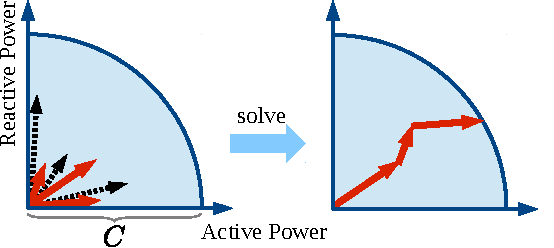
\includegraphics[scale=0.85]{fig/fig-sol-horizontal.pdf}
%	\end{center}
%\caption{The left figure shows the set of all demands $\{S_k(t)\}$. Red vectors represent a feasible solution to {\sc maxPA} such that the total magnitude of the red demands remain within radius $C$ as shown in the right figure.}
%	\label{fig:problem}
%\end{figure}  



%In particular, we will write {\sc maxPA}$[\phi_1,\phi_2]$ for the restriction of problem {\sc maxPA} subject to $\phi_1 \le \max_{k \in {\cal N}}{\rm arg}(S_k(t)) \le \phi_2$, where ${\rm arg}(S_k(t))\ge 0$ for all $k \in {\cal N}$ (see Fig.~\ref{fig:rotate} for an illustration). We remark that in realistic setting of power systems, the active power demand is positive (i.e., $P_k(t) \ge 0$), but the power factor (i.e., $\frac{d^{\rm R}_k}{|S_k(t)|}$) is bounded by a certain threshold \cite{NEC}, which is equivalent to restricting the argument of complex-valued demands. 
%\begin{figure}[!ht]
%	\begin{center}
%		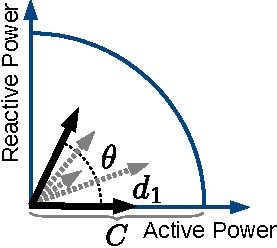
\includegraphics[scale=1]{fig/fig-angle.pdf}
%	\end{center}
%\caption{$\theta$ is the maximum angle between any pair of demands. }
%	\label{fig:rotate}
%\end{figure} 

%For complexity issues, we will need to specify how the input is described. Throughout the paper will assume that each of the demands is given by its real and imaginary components, represented as rational numbers\footnote{we may also consider other representations, such as the {\it polar representation}, and the conversion between the two representations can be done using standard numerical approximations}, and that the capacity parameter $C$ is also rational. 


The generation capacity $C(t)$ could be dynamically varying, and the decisions of load curtailment $(x_k(t))_{k \in {\cal N}}$ need to be determined from time to time. It is assumed that the decisions are triggered at every discrete timeslot $t$. 


\vspace{-5pt}
\subsection{Close-to-optimal Solutions}

Since the exact optimal solutions are computationally hard, this paper focuses on feasible solutions that are close to the optimal solutions. Furthermore, these close-to-optimal solutions are assured with a precise worst-case guarantee on the optimality gap. Some notations are defined as follows to characterize the optimality gap.
\\


\begin{definition}
For clarity, {\sc maxPA} is considered.
Let $ x^\ast_k $ be an optimal solution to {\sc maxPA} and $\OPT \triangleq \sum_{k\in{\cal N}}u_k x^\ast_k$ be the corresponding total valuation.
An approximation solution with $\alpha \in [0, 1]$ worst-case guarantee to {\sc maxPA} is a feasible solution $(\hat{x}_k)_{k \in {\cal N}} \in \{0, 1\}^n$ satisfying %\vspace{-5pt}
\begin{eqnarray}
& &   \displaystyle \sum_{k\in{\cal N}}u_k \hat{x}_k\ge \alpha \cdot \OPT \\
\text{and} & & \displaystyle \Big|\sum_{k\in{\cal N}}S_k \hat{x}_k\Big| \le C \label{C1'}.
\end{eqnarray}
\end{definition}


The worst-case guarantee is called {\em approximation ratio}, which characterizes the ratio between the optimal solution and the approximation solution. When $\alpha = 1$, this implies exact optimal solutions. In the subsequent sections, efficient algorithms are presented with definite worst-case guarantees.

First, a greedy approach is proposed that is capable of determining a close-to-optimal solution rapidly. The worst-case guarantee of this greedy approach depends on the maximum phase angle between any pair of power demand. The smaller phase angle produces a smaller optimality gap. 

Second, a one-dimensional projection algorithm is presented that projects the power demands represented by two-dimensional vector in complex plane to one-dimensional vectors, and utilizes a well-known approximation algorithm from knapsack problem to solve the problem. This approach requires more computations, and a longer running time. However, the worst-case guarantee is superior to that of the greedy approach. 

Finally, a hybrid approach is proposed that harnesses both approaches as a two-stage process, where the greedy approach is firstly utilized rapidly to maintain microgrid stability, and then the one-dimensional projection algorithm is used to improve the decisions, when more response time is permitted.

\vspace{-5pt}
\subsection{Power-off Protection}

It may be undesirable to curtail the load from a customer frequently, as this may cause considerable damages to the electric equipment. To ensure the protection in demand response management, a minimum power-off protection constraint is considered.
\\


\begin{definition}
{\em Minimum power-off protection constraint} ({\sc MPOP}) is a requirement that when a customer's power is curtailed, his power must remain off for a certain minimum duration ($T^{\rm off}_k$) for protection. Namely, if $t$ and $t'$ such that $1 \le t' - t \le  T^{\rm off}_k$, then
\begin{equation}
 x_k(t') = 0 \qquad \mbox{if\ } x_k(t)<x_k(t-1) \label{MPOP}
\end{equation}
\end{definition}

Setting $T^{\rm off}_k = 0$ will disable the power-off protection constraint.
{\sc MPOP} can be applied to both {\sc maxPA} and {\sc minPA} for a period of duration $T$.
\begin{enumerate}

\item
{\em Protection-ensured Valuation-maximizing power allocation problem} ({\sc PEmaxPA}): \vspace{-5pt}
\begin{eqnarray}
\textsc{(PEmaxPA)} & & \displaystyle \max_{x_k(t) \in \{0, 1 \}} \sum_{t=1}^{T} \sum_{k\in{\cal N}}u_k(t) x_k(t) \notag \label{DAP}\\
\text{subject to} & & \displaystyle \Big|\sum_{k\in {\cal N}}S_k(t) x_k(t)\Big| \le C(t) \mbox{\ for all\ } t, \notag  \\
& & \displaystyle  x_k(t') =
0  \mbox{\ if\ } x_k(t)<x_k(t-1) \notag \\
& & \mbox{for\ all\ } t' \mbox{\ such that\ } 1 \le t' - t \le  T^{\rm off}_k  \notag \label{MPOP}
\end{eqnarray}

\item
{\em Protection-ensured Compensation-minimizing power allocation problem} ({\sc PEminPA}): \vspace{-5pt}
\begin{eqnarray}
\textsc{(PEminPA)} & & \displaystyle \min_{x_k(t) \in \{0, 1 \}} \sum_{t=1}^{T} \sum_{k\in{\cal N}}c_k(t) (1-x_k(t)) \notag \label{DAP}\\
\text{subject to} & & \displaystyle \Big|\sum_{k\in {\cal N}}S_k(t) x_k(t)\Big| \le C(t) \mbox{\ for all\ } t, \notag  \\
& & \displaystyle  x_k(t') =
0  \mbox{\ if\ } x_k(t)<x_k(t-1) \notag \\
& & \mbox{for\ all\ } t' \mbox{\ such that\ } 1 \le t' - t \le  T^{\rm off}_k  \notag \label{MPOP}
\end{eqnarray}

\end{enumerate}
The two-stage algorithm is also applied heuristically to the settings considering minimum power-off protection constraint.


\vspace{-5pt}
\section{Efficient Algorithms}\label{sec:algs}


First, note that the problems are invariant, when the arguments of all complex-valued demands are rotated by the same angle (see Fig.~\ref{fig:rotate} for an illustration). 



\begin{figure}[!ht]
	\begin{center} \vspace{-5pt}
		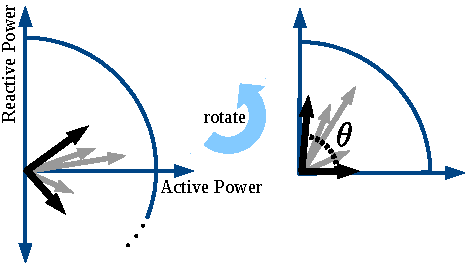
\includegraphics[scale=.8]{fig/rotate.pdf}
	\end{center} \vspace{-5pt}
\caption{Each vector represents a power demand $S_k$. The figure shows that the demands are rotated by the same angle. $\theta$ is the maximum angle between any pair of demands. }
	\label{fig:rotate}
\end{figure} 



Without loss of generality, this paper assumes that one of the demands, say $S_1$ is aligned along the positive real axis, and define a class of sub-problems, by restricting the maximum phase angle $\theta$ (i.e., the argument) that any other demand makes with $S_1$ (see Fig.~\ref{fig:rotate} for an illustration). Note that that in practice $\theta \le \frac{\pi}{2}$, because there are regulations that require electric equipment to conform with a certain maximum power factor (e.g., $\frac{P_k}{|S_k|}\ge 0.8$ \cite{NEC}). For the clarity of presentation, this paper assumes that $P_k \ge 0$ and $Q_k \ge 0$.


\begin{figure}[!htb]
	%\includegraphics[scale=0.3, trim = 0 0 0 0]{fig/normunif.png}
	\centering \vspace{-5pt}
	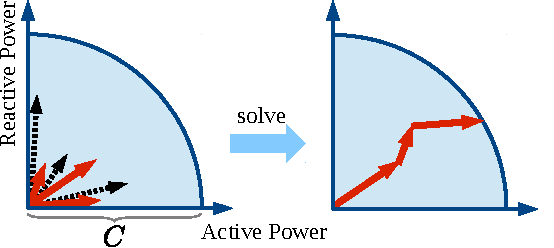
\includegraphics[scale=.7]{fig/fig-sol-horizontal.pdf} \vspace{-5pt}
\caption{The red vectors (thick arrows) represent a feasible solution to {\sc maxPA} such that the total magnitude of the red demands lies within the radius $C$.} \vspace{-5pt}
	\label{fig:problem}
 \end{figure}
 
%\begin{figure}[!ht]
%        \hspace{-10pt}      
%        \begin{subfigure}[h]{0.32\textwidth}\hspace{-10pt}
%                %\includegraphics[scale=0.3, trim = 0 0 0 0]{fig/normunif.png}
%                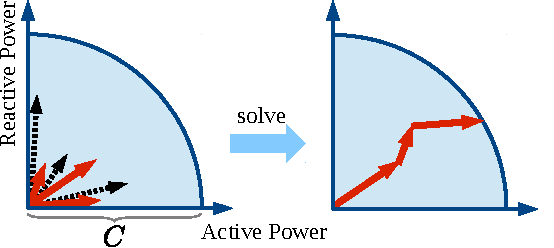
\includegraphics[scale=.7]{fig/fig-sol-horizontal.pdf}
%\caption{The left figure shows a set of all power demands $\{S_k(t)\}$. The red vectors (thick arrows) represent a feasible solution to {\sc maxPA} such that the total magnitude of the red demands remain within radius $C$ as shown in the right figure.}
%              	\label{fig:problem}
%        \end{subfigure}%
%        ~ %add desired spacing between images, e. g. ~, \quad, \qquad etc.
%          %(or a blank line to force the subfigure onto a new line)
%        \begin{subfigure}[h]{0.2\textwidth}
%              %  \includegraphics[scale=0.3, trim = 0 0 0 0]{fig/normnorm.png}
%              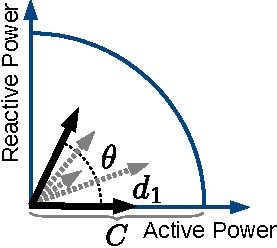
\includegraphics[scale=.7]{fig/fig-angle.pdf}
%\caption{The figure shows demands when all are rotated. The angle  $\theta$ is the maximum  between any pair of demands.\\ }
%	\label{fig:rotate}
%        \end{subfigure}
%\caption{Pictorial representations of {\sc maxPA}.}
%\end{figure}


An allocation $(x_k)_{k \in {\cal N}}$ can be equivalently represented by the set of satisfied customers $X \triangleq \{k\in {\cal N}\mid  x_k=1\}$. For a subset $X \subseteq {\cal N}$, denote $u(X) \triangleq \sum_{k\in X}u_k$.

%In particular, {\em polynomial-time approximation scheme} (PTAS) is an approximation algorithm with $1-\epsilon$ guarantee for any $\epsilon>0$.  The running time of a PTAS is polynomial in the input size for every fixed $\epsilon$, but the exponent of the polynomial might depend on $1/\epsilon$.  One way of addressing this is to define the {\em efficient polynomial-time approximation scheme} (EPTAS), whose running time is the multiplication of a function in $1/\epsilon$ and a polynomial in the input size independent of $\epsilon$. 
%An even stronger notion is a {\em fully polynomial-time approximation scheme} (FPTAS), which requires the running time to be polynomial in both input size and $1/\epsilon$. 










\vspace{-5pt}
\subsection{Greedy Algorithms}

In this section, three simple greedy algorithms are presented. For brevity, consider only the valuation-maximizing problem ({\sc maxPA}). Furthermore, without loss of generality, assume $|S_k| \le C$ for all $k$. 

\begin{enumerate}

\item
{\em Greedy Valuation Algorithm} {\sc(GVA)}: First, sort customers in $\cN = \{1,...,n\}$ by their valuations in a non-increasing order (where ties are broken arbitrarily): \vspace{-5pt}
\begin{equation}
\mbox{if\ }  k \le k', \mbox{\ then\ }  
u_{k} \ge u_{k'}
\end{equation}
Then, select the demands in that order until the capacity constraint ($\big|\sum_{k\in {\cal N}}S_k x_k\big| \le C$) is not satisfied. 


\item 
{\em Greedy Demand Algorithm} {\sc(GDA)}: Similar to {\sc GVA}, but sort the customers by the magnitude of their demands in a non-decreasing order:  \vspace{-5pt}
\begin{equation}
\mbox{if\ }  k \le k', \mbox{\ then\ }  
|S_{k}| \le |S_{k'}|
\end{equation}
Then, select the demands in that order until the capacity constraint ($\big|\sum_{k\in {\cal N}}S_k x_k\big| \le C$) is not satisfied. 

\item 
{\em Greedy Ratio Algorithm} {\sc (GRA)}: Similar to {\sc GVA} and {\sc GDA}, but sort the customers by the efficiency ($\frac{u_k}{|S_k|}$) in a non-increasing order:  %\vspace{-5pt}
\begin{equation}
\mbox{if\ }  k \le k', \mbox{\ then\ }  
\frac{u_k}{|S_k|} \ge \frac{u_{k'}}{|S_{k'}|} 
\end{equation}
Then, select the greedy solution $X$ in that order until the capacity constraint ($\big|\sum_{k\in X}S_k x_k\big| \le C$) is not satisfied. Lastly, return the maximum valuation of two candidate solutions: either greedy solution $X$, or the maximum valuation of a single customer $\arg\max_{k\in \cN}\{ u_k\}$. Fig.~\ref{fig:alge} presents a flowchart of {\sc GRA}.
\end{enumerate}

%\begin{algorithm}[htb!]
%\caption{${\sc GRA} [ \{u_k,S_k(t)\}_{k \in \cN}, C]$}
%\begin{algorithmic}[1]
%\Require customers' utilities and demands $\{u_k,S_k(t)\}_{k\in \cN}$; capacity $C$
%\Ensure $(\frac{1}{2} \sqrt{\frac{\cos \theta + 1}{2}},1)$-solution $\hat{S}$ to \textsc{CKP}
%\State Sort customers in $\cN$ by their efficiency defined by Eqn.~\raf{eq:ef}
%\State $S_1 \leftarrow \varnothing$
%\For{$k \in \cN$} 
%\If{ $\big|\sum_{k' \in S_1} d_{k'} + S_k(t) \big| \le C$} \label{alg:g.feas}
%\State $S_1 \leftarrow S_1 \cup \{k\}$ \label{alg:g.add}
%\EndIf
%\EndFor
%\State Set $S_2 \leftarrow \{\displaystyle {\arg\max}_{k \in \cN   } u_k \}$
%\State Set $\hat{S} \leftarrow \arg\max_{S_1, S_2}\{ u(S_1), u(S_2) \}$ \label{alg:g.max}
%\State \Return $\hat{S}$
%\end{algorithmic}
%\end{algorithm}

\begin{figure}[!ht]
\centering\vspace{-5pt} 
 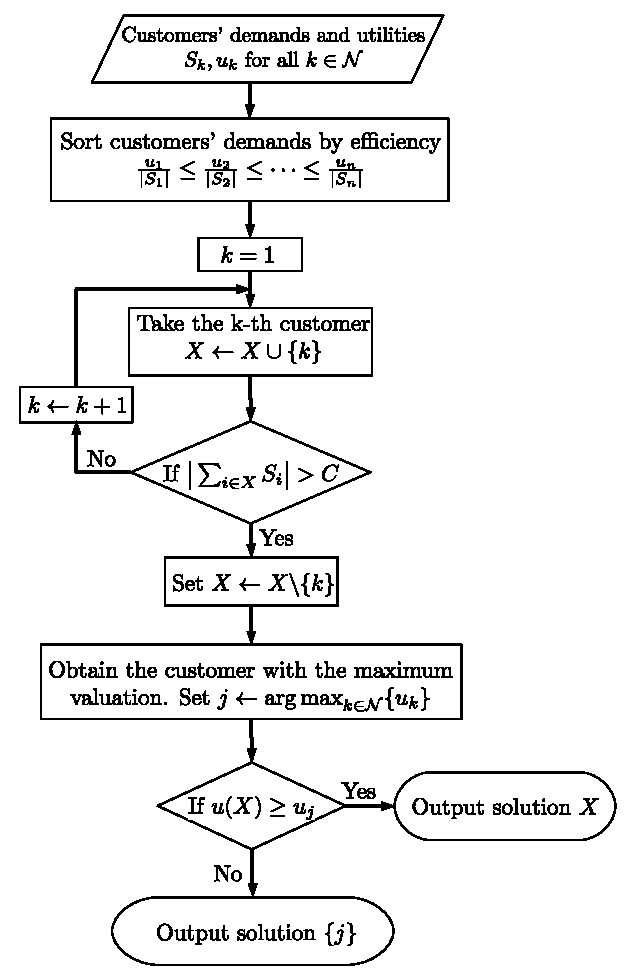
\includegraphics[scale=0.6]{fig/flow-chart-greedy-e.pdf}
\caption{Flow chart for Greedy Ratio Algorithm {\sc (GRA)}.} \vspace{-5pt} 
\label{fig:alge}
\end{figure}

{\sc GVA} and {\sc GDA} are common strategies of load curtailment in practice. 
However, {\sc GRA} possesses a worst-case guarantee, and shows a good empirical ratio with the optimal solutions in simulations.
\\

\begin{customthm}{1} \label{thm:alg-greedy}
Algorithm {\sc GRA} produces a feasible solution within a worst-case guarantee of $\frac{1}{2} \sqrt{\frac{\cos \theta + 1}{2}}$ of the optimal solution of \textsc{maxPA}.
\end{customthm}
\

The worst-case guarantee of {\sc GRA} depends on $\theta$; the smaller the $\theta$, the better guarantee it provides. The basic idea of the proof is discussed in the Appendix. Algorithm {\sc GRA} can be applied to {\sc minPA} by defining the efficiency as ($\frac{c_k}{|S_k|}$). For {\sc minPA}, the worst-case guarantee does not apply, but still shows a good empirical ratio to the optimal solutions by simulations.

\vspace{-5pt} 
\subsection{One-dimensional Projection Algorithm}

In this section, a one-dimensional projection algorithm ({\sc 1DPA}) is presented. Efficient approximation algorithms for classical knapsack problem have been proposed in the literature \cite{KSbook}. However, the problems concerned in this paper belong to a two-dimensional generalization of the one-dimensional classical knapsack problem, for which the immediate application of these algorithms for knapsack problem cannot be applied. A plausible approach is to reduce the two-dimensional problems onto a one-dimensional instance by a proper projection of the power demand vectors to a certain reference vector.

First, consider {\sc maxPA}. The basic idea is to project all power demand vectors onto the $\frac{\pi}{4}$ line (see Fig.~\ref{fig:projection} for an illustration). Namely, create a new vector along the $\frac{\pi}{4}$ line with magnitude $\tilde{S}_k = \frac{P_k + Q_k}{\sqrt{2}}$ for each $S_k = P_k + {\bf i} Q_k$. Then apply the well-known efficient approximation algorithm for the classical knapsack problem \cite{KSbook} (denoted by ${\rm Alg}^{\rm kp}$) on the set $\{\tilde{S}_k\}_{k \in {\cal N}}$ and capacity $\frac{C}{\sqrt{2}}$. 
Lastly, return the maximum valuation of two candidate solutions: either the solution by ${\rm Alg}^{\rm kp}$, or the maximum valuation of a single customer $\arg\max_{k\in \cN} \{u_k\}$. Fig.~\ref{fig:alg0.5} presents a flowchart of {\sc 1DPA}.


\begin{figure}[!ht]
\centering \vspace{-5pt} 
 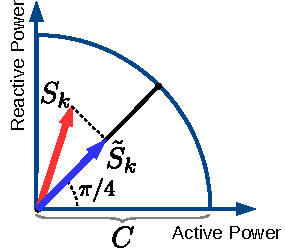
\includegraphics[scale=0.7]{{fig/fig-0.5-alg}.pdf} %\vspace{-5pt} 
 \caption{Each power demand $S_k$ is projected onto the $\frac{\pi}{4}$ line in {\sc 1DPA}.}
\label{fig:projection}
\end{figure} \vspace{-5pt} 




%\begin{algorithm}[htb!]
%\caption{${\cA^\frac{1}{2}} [ \{u_k,S_k(t)\}_{k \in \cN}, C, \epsilon]$}
%\begin{algorithmic}[1]
%\Require Users' utilities and demands $\{u_k,S_k(t)\}_{k\in \cN}$; capacity $C$; accuracy parameter $\epsilon$
%\Ensure $(\frac{1}{2}-\epsilon,1)$-solution $\hat{S}$ to \textsc{CKP}
%\For{$k \in \cN$} 
%\State Set $\tilde{S}_k \leftarrow  \frac{P_k(t)+Q_k(t)}{\sqrt{2}} $
%\EndFor
%\State Set $S_1 \leftarrow {\sc Alg}^{\rm 1d}[(\tilde{S}_k,u_k: k \in \cN),\frac{C}{\sqrt{2}},2\epsilon]$
%\State Set $S_2 \leftarrow \{\displaystyle {\arg\max}_{k \in \cN : S_k(t) \in {\cal D}_2  } u_k \}$
%\State Set $\hat{S} \leftarrow \arg\max_{S_1, S_2}\{ u(S_1), u(S_2) \}$
%\State \Return $\hat{S}$
%\end{algorithmic}
%\end{algorithm}
\begin{figure}[!ht]
\centering \vspace{-5pt} 
 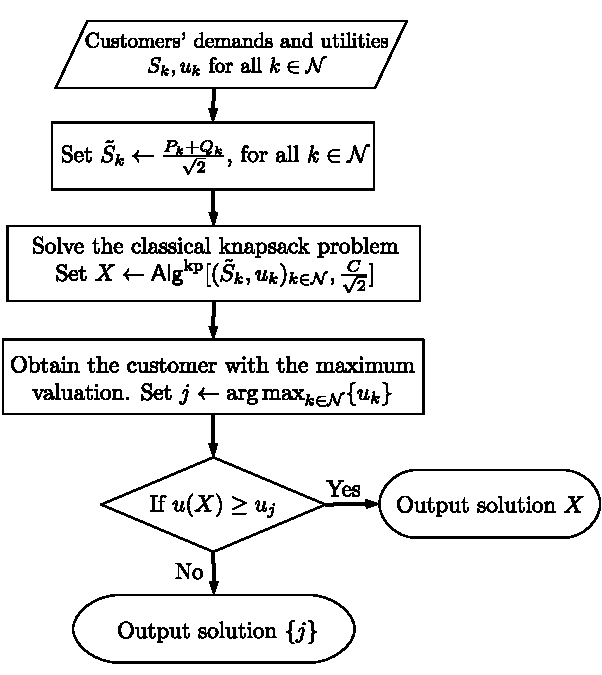
\includegraphics[scale=0.6]{{fig/flow-chart-0.5}.pdf} 
 \caption{Flow chart for One-dimensional Projection Algorithm {\sc (1DPA)}.} %\vspace{-5pt} 
\label{fig:alg0.5}
\end{figure}\vspace{-5pt}


\begin{customthm}{2} \label{thm:1dpa}
Algorithm {\sc 1DPA} produces a feasible solution with a worst-case guarantee $\frac{1}{2}$ with the optimal solution of \textsc{maxPA}.
\end{customthm}
\

Because $\frac{1}{2} \sqrt{\frac{\cos \theta + 1}{2}} \le \frac{1}{2}$, {\sc 1DPA} gives a superior worst-case guarantee than that of {\sc GRA}. The basic idea of the proof is discussed in the Appendix. Algorithm {\sc 1DPA} can be applied to {\sc minPA} by defining the efficiency as ($\frac{c_k}{|S_k|}$). 

Algorithm {\sc 1DPA} can be applied to {\sc minPA} by applying a similar one-dimensional projection approach to reduce the two-dimensional problem into a one-dimensional min-knapsack problem \cite{minKS}.








\iffalse
Now we prove Theorem \ref{thm:2apx}.
\begin{proof}
Let $S^*$ be an optimal solution to C-KP, for which the feasible region is $\cal D$.  Let $S_1^*$, $S_2^*$ be an optimal solution for the subproblem on feasible region ${\cal D}_1$ and ${\cal D}_2$ respectively.  By our observation in Subsection \ref{subsec:pic}, $S_1^*$ is an optimal solution to 1-KP on projected demands and capacity $C/\sqrt{2}$.  Since ${\sc Alg}^{\rm 1d}$ is a $\rho$-approximation algorithm to {\sc 1-KP}, we have $v(S_1)\geq \rho \cdot v(S_1^*)$.  It is also evident that $v(S_2^*)=v(S_2)$.

Next, we analyze the approximation ratio of ${\sc Alg}^{\rm a}$ in three cases.  Here for a subset $S \subseteq K$, we define 
\begin{equation*}
d(S) \triangleq \sum_{k\in S} S_k(t)=\sum_{k\in S} P_k(t)+ {\bf i}\sum_{k\in S} Q_k(t) 
\end{equation*}

\noindent {\bf Case (1): ($\rho$-approximation) } We consider an optimal solution $S^\ast$, such that its sum of demands $d({S^\ast})\in {\cal D}_1$.  

%\begin{proof}
This is an easy case where $v({S^\ast})=v({S_1^\ast})$.  We have $v(S) \ge v(S_1)\ge  \rho \cdot v({S_1^\ast})=\rho \cdot v({S^\ast})$.
%\end{proof}
\vskip 5pt

\noindent {\bf Case (2):  ($\frac{\rho}{1+\rho}$-approximation) } We consider an optimal solution $S^\ast$, such that $d({S^\ast})\in {\cal D}_2$, and there exists an item $j\in S^\ast$ whose demand $d_j\in {\cal D}_2$.  

%\begin{proof}
Let $z \triangleq \sum_{k\in S^\ast\setminus\{j\}} S_k(t)$. Thus, $d({S^\ast})=d_j+z$, i.e., the sum of demands of $S^\ast$ can be written as the sum of a single demand $d_j$ and a subset sum $z$.\footnote{It is possible that $S^{\ast}$ only consists of a single item $j$, in which case our algorithm obviously produces the optimal answer.}  Note that $d_j\in {\cal D}_2$ and $z\in {\cal D}_1$. Otherwise, the projection of $d({S^\ast})=d_j+z$ on the $\frac{\pi}{4}$ line would exceed $2\cdot C/\sqrt{2}>C$.  

Moreover, we have $v({S^\ast\setminus\{j\}}) \le  v({S_1^\ast})$, because $S_1^\ast$ is an optimal solution for feasible region ${\cal D}_1$.  On the other hand, $v_j \le v({S_2})$ since item $j$ with $d_j\in {\cal D}_2$ is a candidate for $S_2$ in our algorithm.  
We obtain:
\begin{equation*}
v({S^\ast})=v_j+v({S^\ast\setminus\{j\}}) \le  v({S_2})+v({S_1^\ast})
\end{equation*}

By the description of our algorithm, the total value of the output solution $v(S)=\max(v({S_1}), v({S_2}))\geq \max(\rho\cdot v({S_1^*}), v({S_2}))= \max(\rho\cdot v({S_1^*}), v({S_2^*}))$.  Now it remains to show that it is further $\geq \frac{\rho}{1+\rho}(v({S_2})+v({S_1^*}))$.

If $\rho\cdot v({S_1^*})\geq v({S_2})$, we have that $v(S)$ is at least 
\begin{equation*}
\rho\cdot v({S_1^*})= \frac{\rho}{1+\rho}(\rho\cdot v({S_1^*})+v({S_1^*}))
\geq \frac{\rho}{1+\rho}( v({S_2})+v({S_1^*}));
\end{equation*}
otherwise, $v(S)$ is at least  
\begin{equation*}
v({S_2})= \frac{\rho}{1+\rho}(v({S_2})+\frac{1}{\rho}v({S_2}))\geq \frac{\rho}{1+\rho}( v({S_2})+v({S_1^*})).
\end{equation*}
%Combining with $\max\{ u(S_1^\ast), u({S_2^\ast})\}\ge \frac{1}{2}\left(u({S_1^\ast})+u({S_2^\ast})\right)$ and $u(S) \ge\rho \cdot \max\{ u(S_1^\ast), u({S_2^\ast})\}$, we get $u(S)\ge \frac{\rho}{2} u({S^\ast})$.

%\end{proof}

\noindent {\bf Case (3): ($\frac{\rho}{2}$-approximation) } We consider an optimal solution $S^\ast$, such that $d({S^\ast})\in {\cal D}_2$, and $S_k(t)\in {\cal D}_1$ for every item $k\in S^\ast$.

%\begin{proof}
First, we let $\tilde{d}(S) \triangleq \sum_{k\in S} \tilde{S}_k$.  The condition on $S^{\ast}$ is equivalent to the following condition on 
projected demands on the $\frac{\pi}{4}$ line: $C/\sqrt{2}<\tilde{d}({S^\ast}) \leq C$, and $\tilde{S}_k \le  C/\sqrt{2}$ for every item $k\in S^\ast$.

We use Lemma \ref{lem:subsetsumA} to show that $d({S^\ast})\in {\cal D}_2$ can be written as the sum of two demand subset sums in ${\cal D}_1$.  Lemma \ref{lem:subsetsumA} is essentially an equivalent statement of this on the projected demands, and will be proved later in this subsection.     

\begin{lemma} \label{lem:subsetsumA}
For a set of $n$ positive real numbers $a_1, ..., a_n$ satisfying $\sum_{i = 1}^n a_i \le C$,  $a_i \le C'$ for all $i$ and $C'\ge C/\sqrt{2}$, there exists a subset $T \subseteq \{1,...,n\}$ such that
\begin{equation*}
\sum_{i \in T} a_i \le C' \mbox{\ \ and \ \ } \sum_{i \in \{1,...,n\} \backslash T} a_i \le C'.
\end{equation*}
\end{lemma}

By Lemma \ref{lem:subsetsumA}, we have $\tilde{d}(T)$ and $\tilde{d}({S^{\ast}\setminus T}) \le  C/\sqrt{2}$ for some subset $T \subseteq S^\ast$. That is, $d(T)  \in {\cal D}_1$ and $d({S^\ast\setminus T}) \in {\cal D}_1$.

Thus, $v(T) \le  v({S_1^\ast})$ and $v({S^\ast\setminus T}) \le  v({S_1^\ast})$.  Moreover, since $v({S^\ast})=v(T)+v({S^\ast\setminus T})$, we have $v({S^\ast}) \le  2v({S_1^\ast})$.  Hence  
\begin{equation*}
v(S) \ge v(S_1)\ge  \rho \cdot v(S_1^\ast)\ge\frac{\rho}{2} v({S^\ast}).
\end{equation*}
%\end{proof}

Combining Cases (1)-(3): $\min\{\rho, \rho/(1+\rho), \rho/2 \} = \rho/2$, we complete the proof of the approximation ratio of ${\sc Alg}^{\rm a}$ as $\rho/2$.
\end{proof}

Finally, we prove Lemma \ref{lem:subsetsumA}:

\begin{proof} 
The case $\sum_{i=1}^{n} a_i\leq C'$ is trivial.  Otherwise, 
let $j$ be the smallest index such that the partial sum exceeds $C'$, i.e., $\sum_{i=1}^{j-1} a_i \le  C'$ and $\sum_{i=1}^{j} a_i>C'$.  Clearly $j \ge 2$ since all $a_i \le  C'$.

Let $x=\sum_{i=1}^{j-1} a_i$, $z=a_j$ and $y = \sum_{i=j+1}^{n} a_i$.  

Note that $\sum_{i = 1}^{n} a_i = x+y+z$.  We already have 
\begin{equation*}
x \le  C',\ \ z \le  C',\ \ 
x+y+z > C' \mbox{\ \ and\ \ } x+z > C'
\end{equation*}

The lemma holds if $y+z \le  C'$, because we can set $T = \{1 ,..., j-1 \}$.  

If $y+z> C'$, then we obtain:
\begin{eqnarray*}
x+y & = & 2(x+y+z)-(x+z)-(y+z)  \\
& < & 2C-2C'\le  (2-\sqrt{2})C  < \frac{C}{\sqrt{2}}\le C'
\end{eqnarray*}
because $x+y+z \le  C$.
Hence, we can set $T = \{1 ,..., j-1, j+1, ..., n\}$.  
\end{proof}
\fi

\vspace{-5pt} 
\subsection{Two-stage Hybrid Approach}

{\sc GRA} can be executed rapidly, as it relies on a greedy approach. However, the worst-case guarantee of {\sc 1DPA} outperforms that of {\sc GRA}. Note that a superior worst-case guarantee does not necessarily imply superior empirical ratio with the optimal solutions in practice. It is possible that some instances of problems may give {\sc GRA} a superior solution to that of {\sc 1DPA}. Therefore, one can obtain an improved solution by selecting the one with the maximum valuation (or the minimum compensation cost) of the candidate solutions from {\sc GRA} and {\sc 1DPA}.

Therefore, a two-stage algorithm ({\sc 2SA}) is proposed to leverage both approaches. The first stage uses {\sc GRA} that is capable of determining a close-to-optimal load curtailment scheme rapidly to maintain microgrid stability. The second stage relies on {\sc 1DPA} that can further improve the optimality solution of the first stage, when more response time is permitted. 

\vspace{-5pt} 
\subsection{Power-off Protection}

The aforementioned algorithms can be applied heuristically to the settings with minimum power-off protection constraint ({\sc MPOP}). At each time $t$, the decision is made with respect to the set of feasible customers $\hat{\cal N}(t)$, who are not restricted by minimum power-off protection constraint. Namely, define \vspace{-5pt} 
\begin{eqnarray}
\hat{\cal N}(t) = \Big\{ k \in {\cal N}& \mid & \mbox{there exists no\ } t' \mbox{\ such that\ } \notag \\
 & & x_k(t')=0 \mbox{\ and\ } t - t' \le  T^{\rm off}_k \Big\}
\end{eqnarray} 
Then, {\sc GRA}, {\sc 1DPA} and {\sc 2SA} are applied to $\hat{\cal N}(t)$ similarly.
%
\subsection{Bi-criteria FPTAS for \textsc{CKP}} 
 

% In this section, we extend our study to the second quadrant (\textsc{CKP$[0,\pi\mbox{-}\varepsilon]$}) for any $\varepsilon > 0$, that is, we assume ${\rm arg}(d_k) \le \pi-\varepsilon$ for all $k \in \cN$. We note that the next section shows that \textsc{CKP$[0, \pi]$} is inapproximable and 
%there is no $(\alpha, 1)$-approximation for \textsc{CKP$[0,\pi \mbox{-} \varepsilon]$}. Therefore, we can at best obtain a bi-criteria approximation, and furthermore the running time should depend on the maximum angle $\phi\triangleq\max_k{\rm arg}(d_k)$.

%For convenience, we let $\theta = \max\{\phi - \frac{\pi}{2},0\}$
%%, such that ${\rm arg}(d_k) \le \theta + \frac{\pi}{2}$ for all $k \in \cN$
% (see Fig.~\ref{f4} for an illustration).
%\begin{figure}[!htb]
%	\begin{center}
%		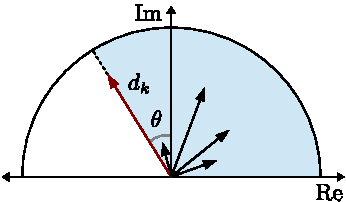
\includegraphics{fig/fig4.pdf}
%	\end{center}
%\caption{All demands lie in the shaded area. We measure $\theta = \phi - \frac{\pi}{2}$ from the imaginary axis.}
%	\label{f4}
%\end{figure}
 

We present a  $(1,1+\epsilon)$-approximation  for \textsc{CKP} denotee by Algorithm {\sc CKP-FPTAS} that is polynomial in both $\frac{1}{\epsilon}$ and $n$ (i.e., FPTAS). This algorithm is illustrated in a previous work~\cite{CEK14CKP}.

% We assume that $\tan \theta$ is bounded polynomial $P(n)\ge 1$ in $n$.
%; as we will see in the next section, without this assumption, a bi-criteria FPTAS is unlikely to exist. 

%Let $\cN_+\triangleq \{k \in \cN \mid d_k^{\rm R} \ge 0\}$ and $\cN_-\triangleq\{k \in \cN \mid d_k^{\rm R} < 0\}$ be the subsets of users with demands in the first and second quadrants respectively. Consider any  solution $S$ to \textsc{CKP$[0,\pi\mbox{-}\varepsilon]$} and define $S_+ \triangleq \{ k \mid d_k^{\rm R} \ge 0, k \in S \}$ and $S_- \triangleq \{ k \mid   d_k^{\rm R} < 0, k \in S \}$ as the subsets of users with demands having non-negative and negative real components respectively. 

The basic idea of Algorithm {\sc CKP-FPTAS} is to enumerate the guessed total projections on real and imaginary axes.% for $S_+^\ast$ and $S_-^\ast$ respectively. 
%We can use $\tan \theta$ to upper bound the total projections for any feasible subset $S$ as follows:
%\begin{align}
% \sum_{k \in S} d_k^{\rm I} \le C, \quad
% \sum_{k \in S_- } - d_k^{\rm R}   \le  C \tan \theta, \quad 
% \sum_{k \in S_+}  d_k^{\rm R}   &\le C(1+ \tan \theta). \label{eq:ubounds}
%\end{align}
We then solve two separate {\sc 2DKP} problems  to find subsets of demands that satisfy the individual guessed total projections. But since {\sc 2DKP} is generally NP-hard, we need to round-up the demands to get a problem that can be solved efficiently by dynamic programming. We show that the violation of the optimal solution to the rounded problem w.r.t. to the original problem is small in $\epsilon$. 

Next, we describe the rounding in detail. First, we define
%\footnote{For a more efficient procedure, we may replace $P(n)$ by $\max\{\tan \theta,1\}$; however, choosing $L$ to depend only on $P(n)$, and thus independent of the demands, will be needed for the truthful mechanism in Sec. \ref{sec:tbp}} 
$L \triangleq \frac{\epsilon C}{n}$, such that the new rounded-up demands $\hat{S_k}$ are defined by:
\begin{equation}
\hat S_k =
\hat S_k^{\rm R} + {\bf i} \hat S_k^{\rm I} \triangleq  
\left\lceil \frac{S_k^{\rm R}}{L} \right\rceil \cdot L + {\bf i} \left\lceil \frac{S_k^{\rm I}}{L} \right\rceil \cdot L
\label{eq:truc}
\end{equation}
Let $\xi$, $\zeta$  be respectively the guessed real and imaginary absolute total projections of the rounded demands in $S^\ast$.
%\begin{equation}
%\xi_+ \triangleq \{ d_k^{\rm R} \mid  k \in S_+ \}, \  \zeta_+ \triangleq \{ d_k^{\rm I} \mid  k \in S_+ \}, \ \xi_- \triangleq \{ - d_k^{\rm R} \mid  k \in S_- \}, \  \zeta_- \triangleq \{ %d_k^{\rm I} \mid  k \in S_- \}
%\end{equation}
Then the possible values of $\xi$ and $\zeta$ are integer mutiples of $L$:
\begin{align}
% \xi \in {\cal A}_+ & \triangleq \left\{0, L, 2L,\ldots,\left\lceil \frac{C (1 + P(n) )}{L} \right\rceil \cdot L\right\},\\
%\xi_- \in {\cal A}_- &\triangleq \left\{0,L, 2L,\ldots, \left\lceil \frac{C \cdot P(n) }{L} \right\rceil\cdot L \right\}, \nonumber \\
\xi, \zeta  \in {\cal A} & \triangleq \left\{0, L, 2L,\ldots,\left\lceil \frac{C}{L} \right\rceil\cdot L.\right\}
\label{eq:grid}
\end{align}
%Note that a feasible guess of total projections should satisfy constraint Eqn.~\raf{C1} for \textsc{CKP}, and thus:
%\begin{equation}\label{eq:sat}
%(\xi_+ - \xi_-)^2 + (\zeta_+ + \zeta_-)^2 \le (1+2\epsilon)^2C^2;
%\end{equation}
%see Lemma~\ref{lem-trunc} below. 
%Step \ref{alg:tight} forces the corresponding selected demands to be tight; otherwise, constraint Eqn.~\raf{C1} could be violated largely. Now, for each guess, we consider solving two {\sc 2DKP} instances separately. The first one with capacities $\xi_+$, $\zeta_+$ and positive demands $\hat d_k, k \in \cN_+$, and the second with $\xi_-,\zeta_-$ and demands in $\cN_-$. 


The next step is to solve the rounded instance exactly. Assume an arbitrary order on $\cN = \{ 1, ..., n\}$. We use recursion to define a 3D table, with each entry ${U}(k,c_1, c_2)$ as the maximum utility obtained from a subset of users $\{1,2,\dots,k\} \subseteq \cN$ with demands $\{\hat{S_1},\hat{S_2},...,\hat{S_k}\}$ that can fit exactly (i.e., satisfies the capacity constraint as an equation) within capacity $c_1$ on the real axis and $c_2$ on the imaginary axis. 

The cells are defined according to the following rules:
\begin{align}
{U}(1,C_1, C_2) &\triangleq  \left\{ \begin{array}{l l}
u_k & \quad \text{if $\hat{P_k} = C_1$ and $\hat Q_k  = C_2$}\\
-\infty &\quad \text{otherwise} \end{array}\right.\label{eq:dyn-rule1}\\
{U}(i+1,C_1, C_2) &\triangleq \max  \left\{ \begin{array}{l}
u_{i+1} + {U}(i, C_1 - \hat P_k, C_2 - \hat Q_k),\\
{U}(i,C_1,C_2)
 \end{array}\right.
 \label{eq:dyn-rule2}
\end{align}

%We denote by {\sc 2DKP-Exact}$[\cdot]$ the algorithm for solving {\sc 2DKP} by dynamic programming.


%\begin{algorithm}[!htb]
%\caption{{\sc CKP-FPTAS} $( \{u_k,d_k\}_{k \in \cN}, C,\epsilon) $}\label{CKP-FPTAS}
%\begin{algorithmic}[1]
%\Require Users' utilities and demands $\{u_k,d_k\}_{k\in \cN}$; capacity $C$; accuracy parameter $\epsilon$
%\Ensure $(1,1+3\epsilon)$-solution $\hat{S}$ to \textsc{CKP$[0,\pi\mbox{-}\varepsilon]$}
%\State $\hat{S} \leftarrow \varnothing$.
%\ForAll {$d_k$ and $k \in \cN$}
%\State Set $\hat d_k \leftarrow \hat d_k^{\rm R} + {\bf i} \hat d_k^{\rm I} $ as defined by \raf{eq:truc}
%\EndFor
%\ForAll {$\xi, \zeta  \in {\cal A}$}
%\If {$\xi^2 + \zeta^2 \le (1+2\epsilon)^2C^2$}\label{cond1}
%\State $ F \leftarrow \text{\sc 2DKP-Exact}(\{u_k,\frac{\hat d_k}{L}\}_{k\in\cN_+}, \frac{\xi}{L},\frac{\zeta}{L})$
%%\State $ F_- \leftarrow \text{\sc 2DKP-Exact}(\{u_k, \frac{-\hat d_k}{L}\}_{k\in \cN_-}, \frac{\xi_-}{L},\frac{\zeta_-}{L})$ 
%%\If{$F_+, F_- \neq \varnothing$} \label{alg:tight}
%\If{$u(F) > u (\hat{S})$}
%\State $\hat{S} \leftarrow  \{F\}$
%\EndIf 
%%\EndIf 
%\EndIf
%\EndFor
%\State \Return $\hat{S}$
%\end{algorithmic}
%\end{algorithm}


%\begin{algorithm}[!htb]
%\caption{{\sc 2DKP-Exact} $( \{u_k,\hat d_k\}_{k \in \cN'}, C_1,C_2) $}
%\begin{algorithmic}[1] 
%\Require Users' utilities and integer demands $\{u_k,\hat d_k\}_{k\in \cN'}$; integer capacities $C_1,C_2$
%\Ensure A utility-maximizing subset of satisfiable users $\subseteq \cN'$ subject to capacity constraints defined by $C_1,C_2$
%\State Create a 3D table of size $|\cN'| \times (C_1+1) \times (C_2+1)$, with each entry ${U}(k,c_1, c_2)$ according to: 
%\begin{align}
%{U}(1,c_1, c_2) &\triangleq  \left\{ \begin{array}{l l}
%u_1 & \quad \text{if $\hat d_1^{\rm R} = c_1$ and $\hat d_1^{\rm I}  = c_2$}\\
%-\infty &\quad \text{otherwise} \end{array}\right.\label{eq:dyn-rule1}\\
%U(k, 0, 0) &\triangleq 0\\
% U(k, c_1', c_2') &\triangleq -\infty\text{ for all }c_1'<0 \text{ or } c_2'<0\\
%{U}(k,c_1, c_2) &\triangleq \max  \Big\{ 
%u_{k} + {U}(k-1, c_1 - \hat d_k^{\rm R}, c_2 - \hat d_k^{\rm I}), \nonumber\\
%& \qquad \qquad {U}(k-1,c_1,c_2) \Big\}
% \label{eq:dyn-rule2}
%\end{align}
%\State Create a 3D table of size $|\cN'| \times C_1 \times C_2$, with each each entry ${\cI}(k,c_1, c_2)$ according to: 
%
%\begin{align}
%\cI(1,c_1, c_2) &\triangleq \left\{\begin{array}{l l}
%\{1 \}& \ \text{if $U(1,c_1,c_2) = u_1$}\\
%\varnothing & \ \text{otherwise} 
%\end{array}\right.\\
%%%%%%%%%%%%
%{\cI}(k,c_1, c_2) &\triangleq  \left\{ \begin{array}{ll}
%{\cI}(k-1,c_1, c_2) &\\
% \qquad \text{if ${U}(k,c_1, c_2) = {U}(k-1, c_1, c_2)$} \\
%%
%{\cI }(k-1,c_1- \hat d_k^{\rm R}, c_2- \hat d_k^{\rm I}) \cup \{ k \} \\
%  \qquad \text{if } {U}(k,c_1, c_2) = u_{k} + \\\qquad \qquad {U}(k-1, c_1 - \hat d_k^{\rm R}, c_2 - \hat d_k^{\rm I}) & \\
%\end{array}\right.
%%%%%%%%%%%
% \label{eq:dyn-rule3}
%\end{align}
%\State \Return $\displaystyle {\cI}(|\cN'|,C_1,C_2)$.
%\end{algorithmic}
%\end{algorithm}


\begin{theorem}\label{thm:bptas}
Algorithm {\sc CKP-FPTAS} is $(1,1+3\epsilon)$-approximation for \textsc{CKP$[0,\pi\mbox{-}\varepsilon]$} and its running time is polynomial in both $n$ and $\frac{1}{\epsilon}$.
\end{theorem}


\iffalse
\begin{proof}
First, the running time is proportional to the number of guesses, upper bounded by $O(\frac{1}{\epsilon^4} n^{4} P^6(n))$. For each guess, {\sc 2DKP-Exact} constructs a table of size at most $O(\frac{1}{\epsilon^2} n^3 P^4(n))$. Since we assumed $P(n)$ is polynomial in $n$, the total running time is polynomial in $n$ and $\frac{1}{\epsilon}$.

To show the approximation ratio of 1, we note {\sc CKP-FPTAS} enumerates over all possible rounded projections subject to the capacity constraint in {\sc CKP} and that {\sc 2DKP-Exact} returns the exact optimal solution for each rounded problem. In particular, by Lemma \ref{lem-trunc} one of the choices would be rounded projection for the optimum solution $S^\ast$.   
It remains to show that the violation of the returned solution is small in $\epsilon$. This is given in Lemma~\ref{lem-trunc2} below, which shows that the solution $\hat S$ to the rounded problem violates the capacity constraint by only a factor at most $(1+3\epsilon)$. 
\end{proof}

%In fact, $\epsilon$ is inversely proportional to $\theta$. The larger $\theta$ the smaller $\epsilon$ is required for maintaining the precision. This can be observed from Eqn.~\raf{lem1-p2}.

For any set $S\subseteq\cN$, let us write $D_+(S)\triangleq\sum_{k\in S_+}P_k$, $D_-(S)\triangleq\sum_{k\in S_-}-P_k$, $D_I(S)\triangleq\sum_{k\in S}Q_k$, $\hat D_+(S)\triangleq\sum_{k\in S_+} \hat P_k$, $\hat D_-(S)\triangleq\sum_{k\in S_-} -\hat P_k$, and $\hat D_I(S)\triangleq\sum_{k\in S}\hat Q_k$. Then by \raf{eq:truc} and the fact that $x \le t \lceil \frac{x}{t} \rceil  \le x + t$ for any $x,t$ such that $t>0$, we have 
\begin{eqnarray}\label{eq:bds}
&\max\{\hat D_+(S)-L|S|,0\}\le D_+(S)\le \hat D_+(S),~~~\max\{\hat D_-(S)-L|S|,0\}\le D_-(S)\le \hat D_-(S), \nonumber \\ & \max\{\hat D_I(S)-L|S|,0\}\le D_I(S)\le\hat D_I(S).
\end{eqnarray}

\begin{lemma}
For any optimal solution $S^*$ to \textsc{CKP$[0,\pi\mbox{-}\varepsilon]$}, $L\triangleq \frac{\epsilon C}{nP(n)}$ and $\epsilon> 0$, we have
\begin{equation}
 \left( \sum_{k \in S^*} \hat d_k^{\rm R} \right)^2 +  \left(\sum_{k \in S^*} \hat   d_k^{\rm I} \right)^2  \le C^2 ( 1 + 2\epsilon)^2 .
 \label{eq:lem}
\end{equation}
 \label{lem-trunc}
\end{lemma}
\begin{proof}
%First, we note that any optimal solution $S^*$ satisfies constraint Eqn.~\raf{C1}:
%\begin{equation}
%\left(\sum_{k\in S^*} d_k^{\rm R} \right)^2 + \left( \sum_{k \in S^* } d_k^{\rm I}\right)^2 \le C^2
%\label{eq:C1}
%\end{equation}


Using~\raf{eq:bds},
\begin{align}
\left( \sum_{k \in S^*} \hat d_k^{\rm R} \right)^2 +  \left(\sum_{k \in S^*} \hat d_k^{\rm I} \right)^2 &=\left(\hat D_+(S^*)- \hat D_-(S^*)\right)^2 +  \hat D_I^2(S^*)\nonumber\\
&=\hat D_+^2(S^*)+\hat D_-^2(S^*)-2\hat D_+(S^*)\hat D_-(S^*)+\hat D_I^2(S^*)\nonumber\\ 
&\le (D_+(S^*)+nL)^2+(D_-(S^*)+nL)^2-2D_+(S^*) D_-(S^*)+(D_I(S^*)+nL)^2\nonumber\\
&=(D_+(S^*)-D_-(S^*))^2+D_I^2(S^*)+2nL (D_+(S^*)+D_-(S^*)+D_I(S^*))+3n^2L^2\nonumber\\
&= \left(\sum_{k\in S^*} d_k^{\rm R} \right)^2 + \left(\sum_{k\in S^*} d_k^{\rm I}  \right)^2 +2nL\left(\sum_{k\in S^*}|d_k^{\rm R}|+\sum_{k\in S^*}d_k^{\rm I}\right)+3n^2L^2\nonumber\\
&\le C^2 + 4nL (P(n)+1) C + 3n^2L^2 = C^2 + 4 \epsilon C^2 + 3\epsilon^2 C^2/(1+P(n))^2\nonumber \\ &\le C^2 (1+4\epsilon + \epsilon^2)\le C^2(1+2\epsilon)^2\label{lem1-p2}.
\end{align}
\end{proof}

\begin{lemma}\label{lem-trunc2}
Let $\hat S$ be the solution returned by {\sc CKP-FPTAS}. Then $|\sum_{k\in\hat S}d_k|\le(1+3\epsilon) C$. 
\end{lemma}
\begin{proof}
As in~\raf{lem1-p2},
\begin{align}\label{eq:ee1}
\left( \sum_{k \in \hat S} d_k^{\rm R} \right)^2 +  \left(\sum_{k \in \hat S} d_k^{\rm I} \right)^2 &=\left(D_+(\hat S)- D_-(\hat S)\right)^2 +  D_I^2(\hat S)\nonumber\\
&=D_+^2(\hat S)+D_-^2(\hat S)-2D_+(\hat S)D_-(\hat S)+D_I^2(\hat S).
\end{align} 
If both $\hat D_+(\hat S)$ and $\hat D_-(\hat S)$  are less than $nL$, then the R.H.S. of \raf{eq:ee1} can be bounded by 
\begin{align}\label{eq:ee2}
&\hat D_+^2(\hat S)+\hat D_-^2(\hat S)+\hat D_I^2(\hat S)
\le\hat D_+^2(\hat S)+\hat D_-^2(\hat S)-2\hat D_+(\hat S)\hat D_-(\hat S)+2n^2L^2+\hat D_I^2(\hat S)\nonumber\\
&=(\hat D_+(\hat S)-\hat D_-(\hat S))^2+\hat D_I^2(\hat S)+2n^2L^2.
\end{align}
Otherwise, we bound the R.H.S. of \raf{eq:ee1} by
\begin{align}\label{eq:ee3}
&\hat D_+^2(\hat S)+\hat D_-^2(\hat S)-2(\hat D_+(\hat S)-nL)(\hat D_-(\hat S)-nL)+\hat D_I^2(\hat S)\nonumber\\
&=(\hat D_+(\hat S)-\hat D_-(\hat S))^2+\hat D_I^2(\hat S)+2nL(\hat D_+(\hat S)+\hat D_-(\hat S))-2n^2L^2.
\end{align}
Since $\hat S=F_+\cup F_-$ is obtained from feasible solutions $F_+$ and $F_-$ to $\text{\sc 2DKP-Exact}(\{u_k,\hat d_k/L\}_{k\in\cN_+}, \xi_+/L,\zeta_+/L)$
 and $\text{\sc 2DKP-Exact}(\{u_k,-\hat d_k/L\}_{k\in \cN_-}, \xi_-/L,\zeta_-/L)$, respectively, and  $\xi_+ , \xi_-,\zeta_+, \zeta_-$ satisfy the condition in Step~\ref{cond1}, it follows from \raf{eq:ee1}-\raf{eq:ee3} that
\begin{align*}
\left( \sum_{k \in \hat S} d_k^{\rm R} \right)^2 +  \left(\sum_{k \in \hat S} d_k^{\rm I} \right)^2 &\le \left( \sum_{k \in \hat S} \hat d_k^{\rm R}\right)^2 +  \left(\sum_{k \in \hat S}\hat d_k^{\rm I} \right)^2+2nL\sum_{k \in \hat S_-} |\hat d_k^{\rm R}|+2n^2L^2\nonumber\\
&=(\xi_+ - \xi_-)^2 + (\zeta_+ + \zeta_-)^2 + 2nL\xi_-+2n^2L^2\nonumber\\
&\le \left((1+2\epsilon)^2C^2 +2n\frac{\epsilon}{n(P(n)+1)} C^2 + 2n^2\frac{\epsilon^2}{n^2(P(n)+1)^2}\right)C^2\\
&\le \left((1+2\epsilon)^2 +\epsilon + \frac{\epsilon^2}{2}\right)C^2\le (1+3\epsilon)^2C^2.
\end{align*}
\end{proof}

\iffalse
\begin{corollary}
For any $(\alpha, \beta)$-approximation algorithm of \textsc{CKP$[0,\pi\mbox{-}\varepsilon]$} using truncated demands $\hat d_k$, we have $(\alpha, \beta (1+\epsilon))$-approximation for original demands $d_k$.
\label{cor} 
\end{corollary}
This follows immediately from Lemma~\ref{lem-trunc}. The approximation ratio $\alpha$ remains the same since any optimal $S^*$ is also feasible in the new instance within a violation of $(1+\epsilon)$.
\fi

\fi

\vspace{-5pt} 
\section{Simulations}\label{sec:sims}

This section presents the simulation results for corroborating the performance of the proposed algorithms in diverse settings.

\vspace{-5pt} 
\subsection{Settings}

The simulations are based on a microgrid setting with a number of customers, each having a power demand and valuation generated according to a probability preference model. The customers may suffer from a reduction of generation capacity occasionally. The appearances and levels of reduction vary according to a stochastic process model.  

The model is designed to resemble  a real-world scenario, where the microgrid has a total capacity $C$ up to 2MVA connecting to residential customers (with relatively small demand) and industrial customers (with considerably large demand).

The algorithms ({\sc GVA}, {\sc GDA}, {\sc GRA}, {\sc 1DPA}) are applied to both valuation-maximizing and compensation-minimizing problems. 
The simulations were evaluated using 2 Quad core Intel Xeon CPU E5520s 2.21 GHz processors. The algorithms were implemented using C and Python programming languages and a standard random number generation library.
Each customer's reactive power demand equals to $ Q_k = \tan (\phi) \cdot P_k $, where $\phi$ is the phase angle between the reactive and apparent powers. %, and $\phi \in [0, 36]$ according to Electrical Power Engineering standards \cite{citation02}.

\vspace{-5pt} 
\subsection{Scenarios}

Diverse scenarios are considered in the following aspects.

\noindent
i) Power demands:
\begin{enumerate}

\item {\em Full (F) power}: The power demand of each customer can have both non-negative active power ($P_k \ge 0$) and non-negative reactive power ($Q_k \ge 0$).

\item {\em Active (A) power only}: The power demand of each customer can have non-negative active power ($P_k \ge 0$) but zero reactive power ($Q_k = 0$).

\end{enumerate}

\noindent
ii) Valuation/Compensation-demand correlation:
\begin{enumerate}

\item {\em Correlated (C)}: The valuation/compensation of each customer is a function of the power demand:
\begin{equation}\label{eq:valuationfunction}
u_k({|S_k|}) = a({|S_k|})^2 + b{|S_k|} + c 
\end{equation}
where $a > 0, b, c \ge 0$ are constants.

\item {\em Uncorrelated (U)}: The valuation/compensation of each customer is independent of the power demand and is generated randomly from $[0, a({|S_k|})^2 + b{|S_k|} + c]$.

\end{enumerate}

\noindent
iii) Customer types
\begin{enumerate}

\item {\em Industrial (I) customers}: Customers have big active power demands ranging from 300KW up to 1MW.

\item {\em Residential (R) customers}: Customers have small active power demands ranging from 500W to 5KW.

\item {\em Mixed (M) customers}: Customers have a mix of both industrial and residential customers

\end{enumerate}
In the following, a scenario is represented by the acronyms of the types. For example, scenario ACI stands for the one with industrial customers, zero reactive power demands and valuations/compensations-demand correlation.\\

\iffalse
{\em Valuation Model:} 

When the customer's valuation/compensation $u_k$ is correlated with its demand, it is calculated using the valuation function $u_k(|S_k|)$, which indicates the cost of consuming $S_k$ units of energy. We make the following assumptions:\\

\begin{enumerate}

\item
The valuation function is increasing based on the
consumed energy capacity. In other words, for each $k \in {\cal N}$, we have
\begin{center}
${u_k}({|S_k|}) \le {u_k}({{|S'_k|}}), \forall$   $ {|S_k|} \le {{|S'_k|}}$
\end{center}


\item The valuation function is strictly convex. For each  $k \in {\cal N} $, any $0 \le \alpha \le 1$, and ${|S_k|},{|S'_k|} \ge 0$, we have
\begin{center}
$u_k(\alpha |S_k| + (1 - \alpha)|S'_k|) \le \alpha u_k(|S_k|) + (1 - \alpha)u_k(|S'_k|)$
\end{center}
\end{enumerate}
\vspace{3mm}
Among various valuation functions that satisfy the aforementioned assumptions in this paper we use the following quadratic valuation function 
\begin{equation}
\label{eq:valuationfunction}
u_k({|S_k|}) = a({|S_k|})^2 + b{|S_k|} + c 
\end{equation}
where $a > 0, b, c \ge 0$ are pre-determined constants.\\

\fi


\vspace{-5pt}
\subsection{Results}


%In general, {\sc 1DPA}'s performance, in terms of the running time and maximized valuation, varies for different input values of $\epsilon$, that is the higher the $\epsilon$ the higher the running time and the lower the maximized valuation and vice versa. In our simulations the $\epsilon$ value for {\sc 1DPA} algorithm  was set to $10^{-18}$ in order to have as accurate results as possible but keep the running time up to 3 minutes. 

A summary of the simulation results for each the scenario is shown in Table \ref{algorithmscomparison}, which indicate most superior algorithm in the respective scenario. Specifically, fours scenarios are highlighted in Figs.~\ref{fig:scenarioaurfcm}-\ref{fig:scenariofuracm}

\begin{table}[h]
\renewcommand{\arraystretch}{2}
\centering \vspace{-5pt}
\begin{tabular}{lc|l|l|l|l|}
\cline{3-6}
 & \multicolumn{1}{l|}{} & \multicolumn{2}{c|}{F} & \multicolumn{2}{c|}{A} \\ \hhline{~~|-|-|-|-|} %\cline{3-6} 
 & \multicolumn{1}{l|}{} & \multicolumn{1}{c|}{C} & \multicolumn{1}{c|}{U} & \multicolumn{1}{c|}{C} & \multicolumn{1}{c|}{U} \\ \hline
\multicolumn{1}{|c|}{\multirow{2}{*}{{\sc maxPA}}} & R & GRA & GRA & \cellcolor[gray]{.8} 1DPA & \cellcolor[gray]{.8} 1DPA \\ \hhline{|~|-|-|-|-|-|} % \cline{2-6} 
\multicolumn{1}{|c|}{} & M & GDA & \cellcolor[gray]{.8}1DPA &\cellcolor[gray]{.8} 1DPA &\cellcolor[gray]{.8}  1DPA \\ \hline
\multicolumn{1}{|l|}{\multirow{2}{*}{\sc minPA}} & R & GRA & GRA & \cellcolor[gray]{.8} 1DPA &\cellcolor[gray]{.8}  1DPA \\ \hhline{|~|-|-|-|-|-|}% \cline{2-6} 
\multicolumn{1}{|l|}{} & M & GDA & \cellcolor[gray]{.8}  1DPA & \cellcolor[gray]{.8} 1DPA & \cellcolor[gray]{.8}  1DPA \\ \hline
\end{tabular} \vspace{-5pt}
\caption{The results of simulations in each scenario. Each cell of the table indicates the most superior algorithm in the respective scenario.}
\label{algorithmscomparison}
\end{table}

\vspace{-5pt}
\subsubsection{Empirical Ratios with Optimal Solutions}~\\

\begin{figure}[!htb]\vspace{-5pt}
	\begin{center}
		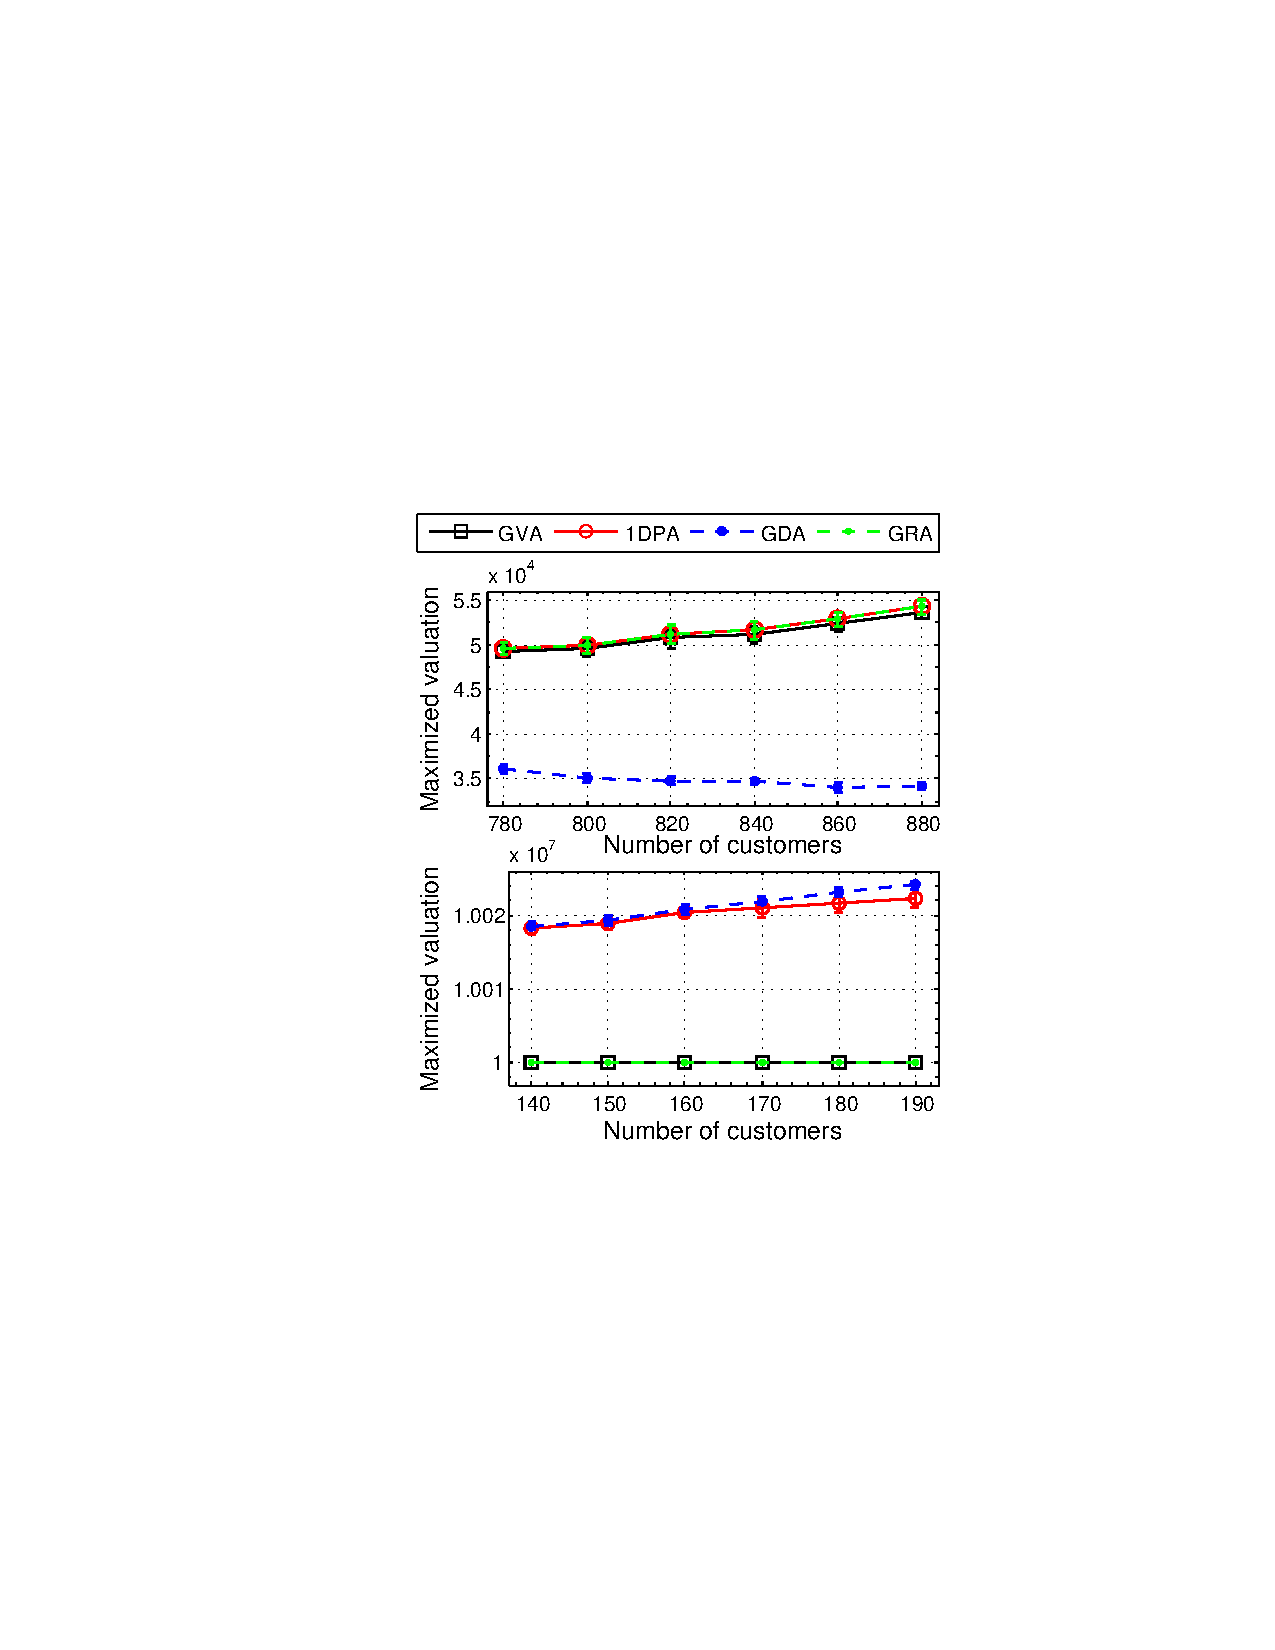
\includegraphics[scale=0.7]{fig/4_5.pdf}
	\end{center}\vspace{-5pt}
\caption{{\sc GVA}, {\sc GDA}, {\sc GRA}, {\sc 1DPA} apply to {\sc maxPA} for scenarios AUR and FCM on top and bottom respectively.}
	\label{fig:scenarioaurfcm}
\end{figure} 

 When customers' reactive demand $Q_k$ is not taken into account, {\sc maxPA} and {\sc minPA} for {\sc 1DPA}  become a simple classical knapsack problem. In fact, in that case the maximized valuation and minimized compensation by {\sc 1DPA} is considerably close to the possible optimal value. This can be seen from Fig.~\ref{fig:scenarioaurfcm} and Table \ref{algorithmscomparison}, which show that {\sc 1DPA} algorithm outperforms all greedy algorithms mentioned in this paper.\\

On the other hand, when customers' reactive demand is considered,  {\sc maxPA} and {\sc minPA} become computationally complex problems for {\sc 1DPA}. In this case {\sc GVA}, {\sc GDA}, {\sc GRA}, and {\sc 1DPA}'s performance varies for these cases when the customers are only residential and when there is a mix of residential and industrial customers as indicated in Fig.~\ref{fig:scenariofuracm} and Table \ref{algorithmscomparison}.

To sum up, the aforementioned simulations show that two key factors, namely the correlation between valuation/compensation and demand, and customers' apparent power, have a substantial impact on the performance of {\sc GVA}, {\sc GDA}, {\sc GRA}, and {\sc 1DPA}.

\begin{figure}[!htb]\vspace{-5pt}
	\begin{center}
		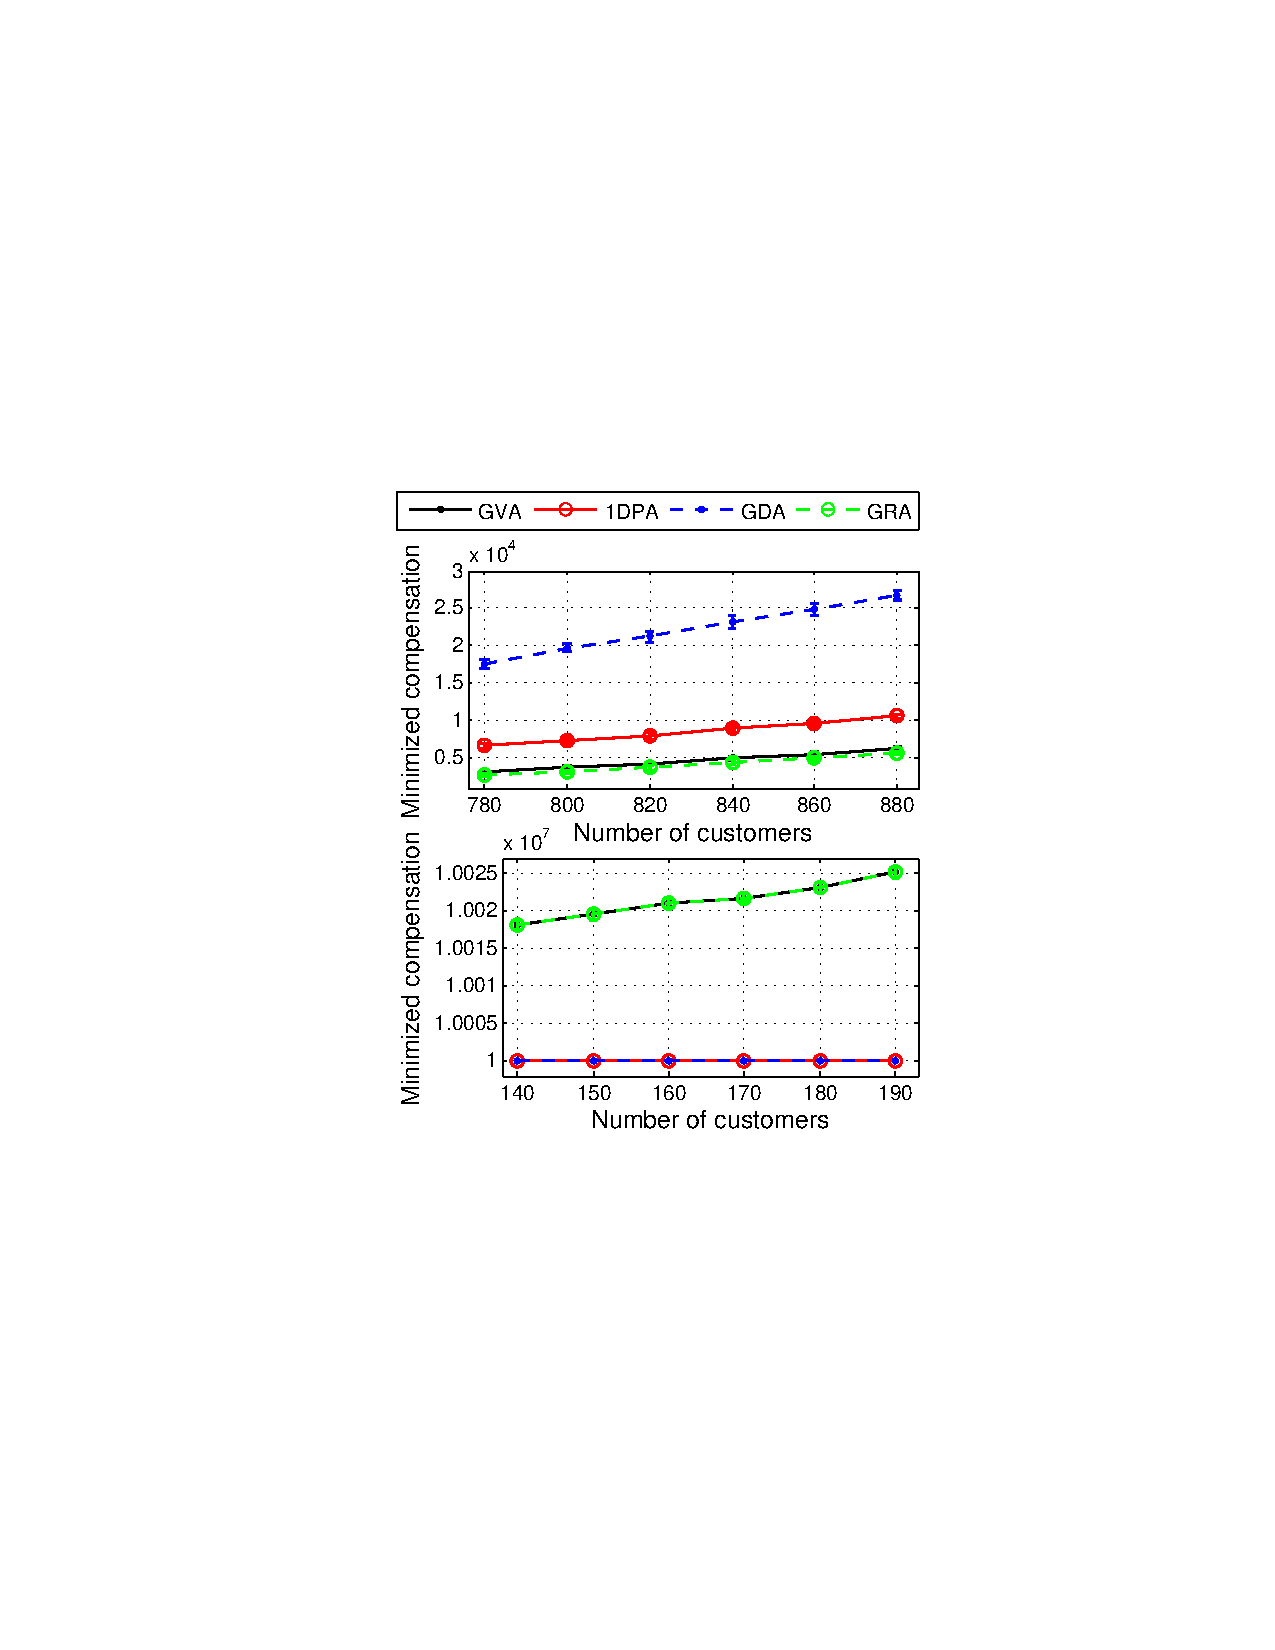
\includegraphics[scale=0.7]{fig/1_8.pdf}
	\end{center}\vspace{-5pt}
\caption{{\sc GVA}, {\sc GDA}, {\sc GRA}, {\sc 1DPA} apply to {\sc minPA} for scenarios FUR and ACM on top and bottom respectively.}
	\label{fig:scenariofuracm}
\end{figure} 

The importance of the load (i.e.,  the priority and the benefit to the system) are among various fundamental factors that should be carefully considered when planning a load curtailment algorithm \cite{466502}. The conventional load curtailment strategies used in power grids (i.e., curtailing loads simply according to the ascending order of priorities \cite{5348255,6493097}), are basically {\sc GVA}, when valuations reflect the priorities.

For the case when the microgrid customers have strictly defined priorities and customers with high priorities are of critical importance and should never be curtailed, the {\sc GVA} is an effective algorithm. Nevertheless, the analysis of the results shows that when the loads have the same or no priority like that in the simulations, in such cases the {\sc GVA} does not produce high valuation or low compensation cost solutions, which can be seen in Table \ref{algorithmscomparison}.\\

 \vspace{-5pt}
\subsubsection{Running Time}
\hspace{2cm}
\begin{figure}[!htb]\vspace{-5pt}
	\begin{center}
		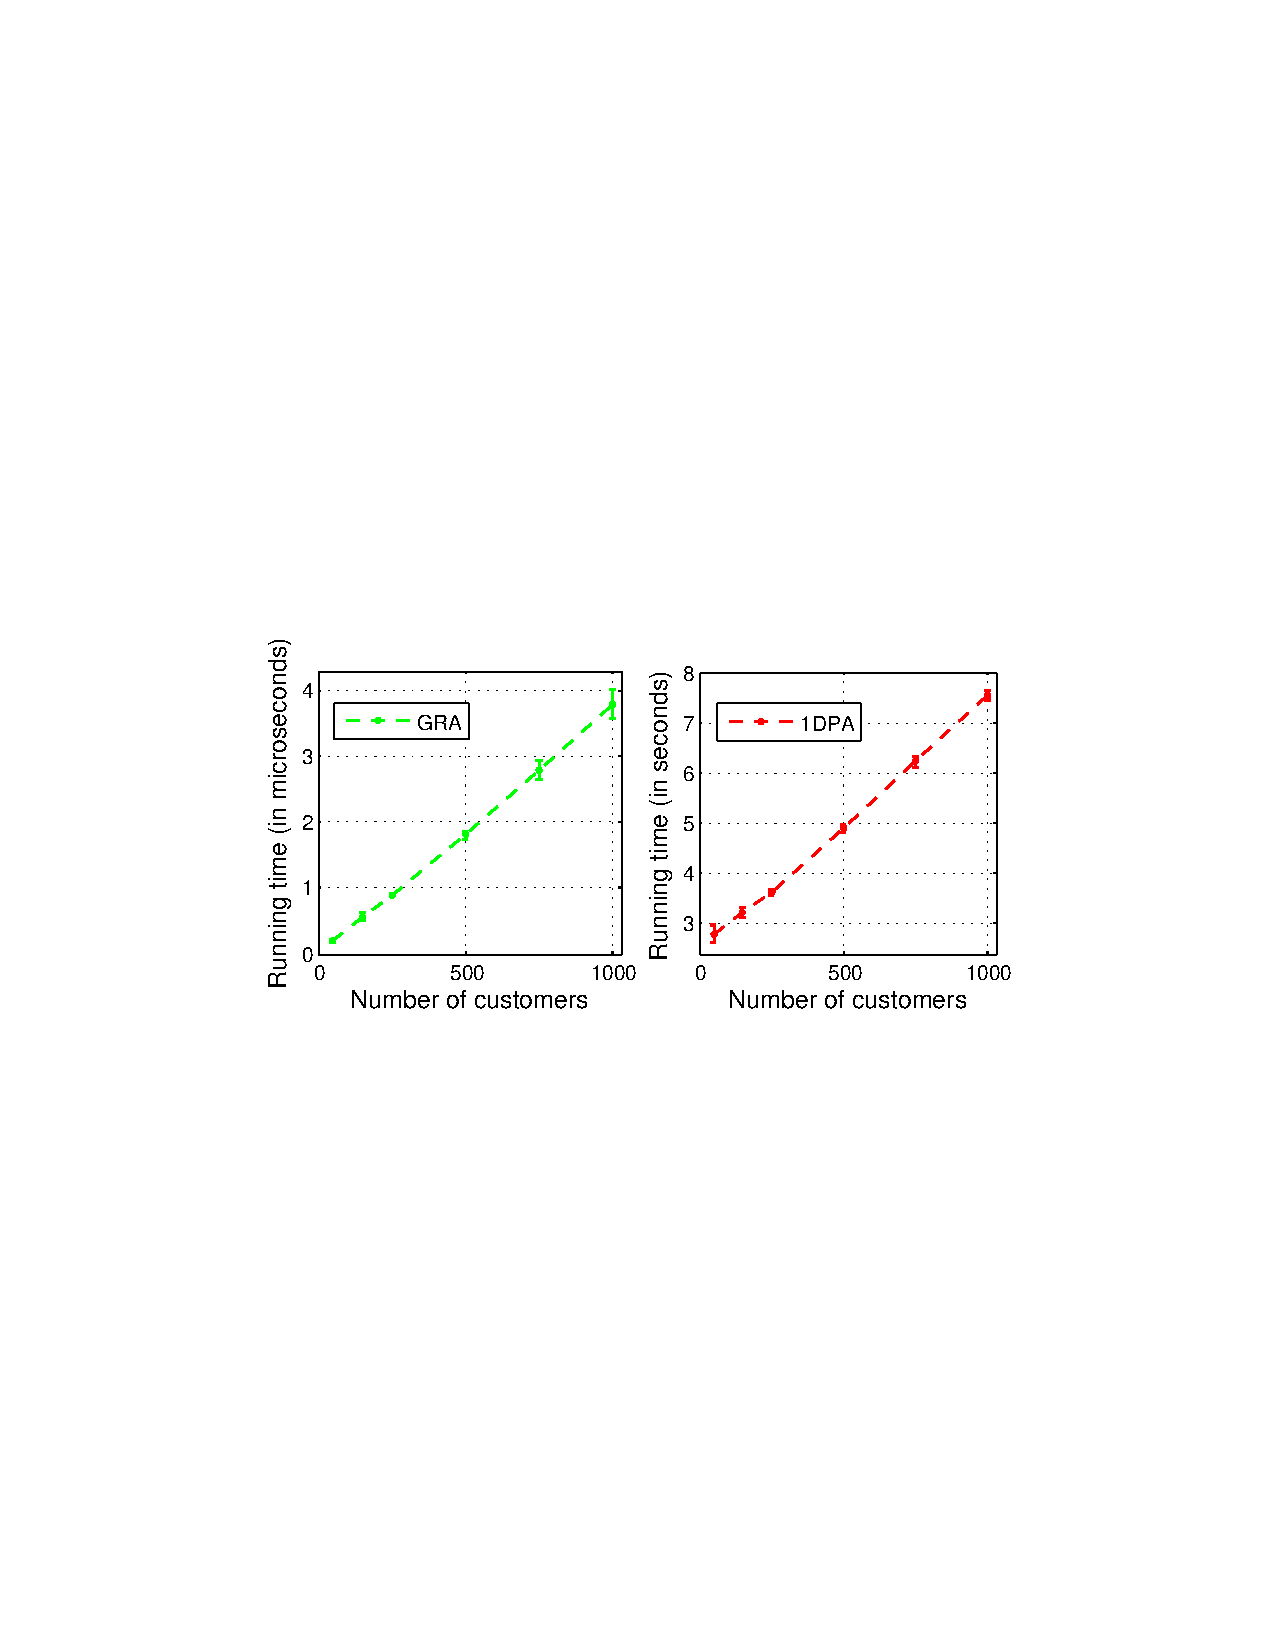
\includegraphics[scale=0.55]{fig/rt.pdf}
	\end{center}\vspace{-5pt}
\caption{The running time of {\sc 1DPA} and {\sc GRA}.}
	\label{fig:rt}
\end{figure}



\begin{figure}[!htb]\vspace{-5pt}
	\begin{center}
		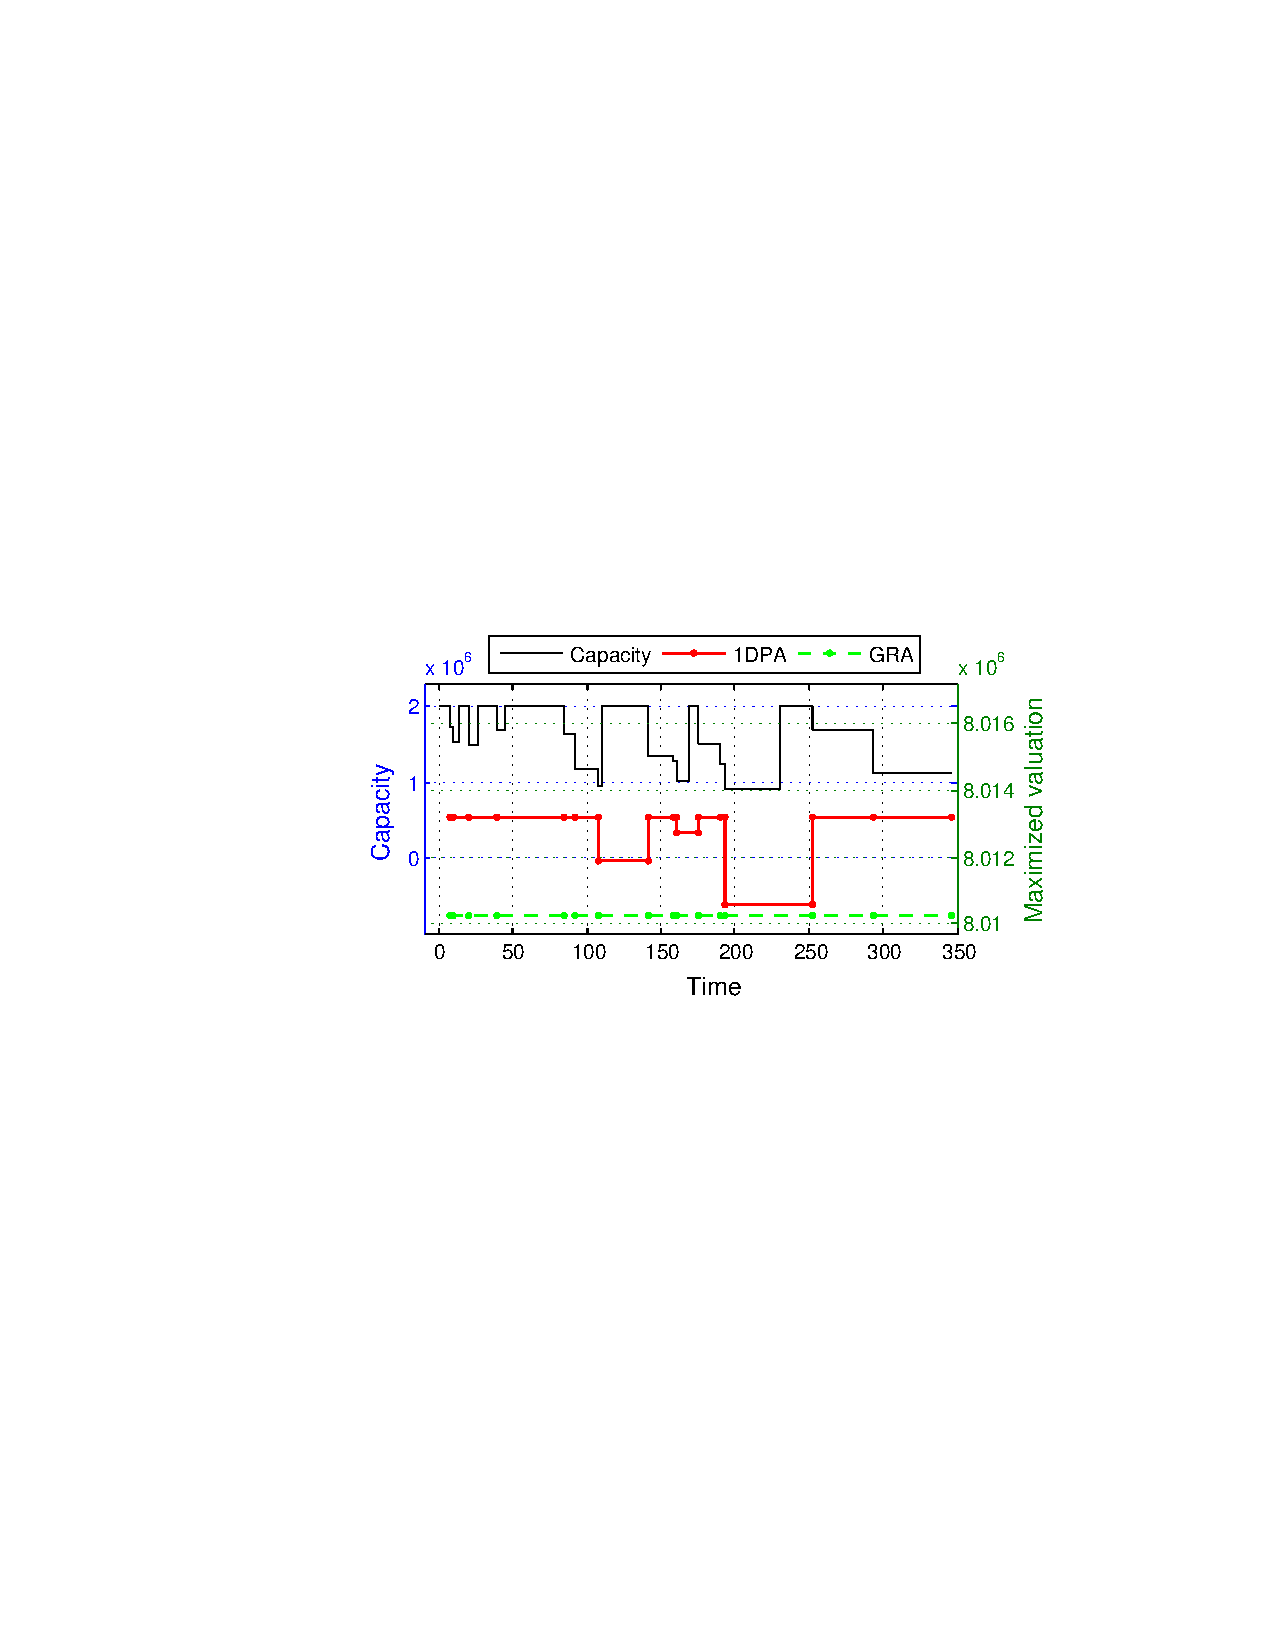
\includegraphics[scale=0.6]{fig/maxPa.pdf}
	\end{center}\vspace{-5pt}
\caption{{\sc 1DPA} and {\sc GRA} apply to {\sc maxPA} without power-off protection constraint for Scenario AUM.}
	\label{fig:maxpa}
\end{figure}

\begin{figure}[!htb]\vspace{-5pt}
	\begin{center}
		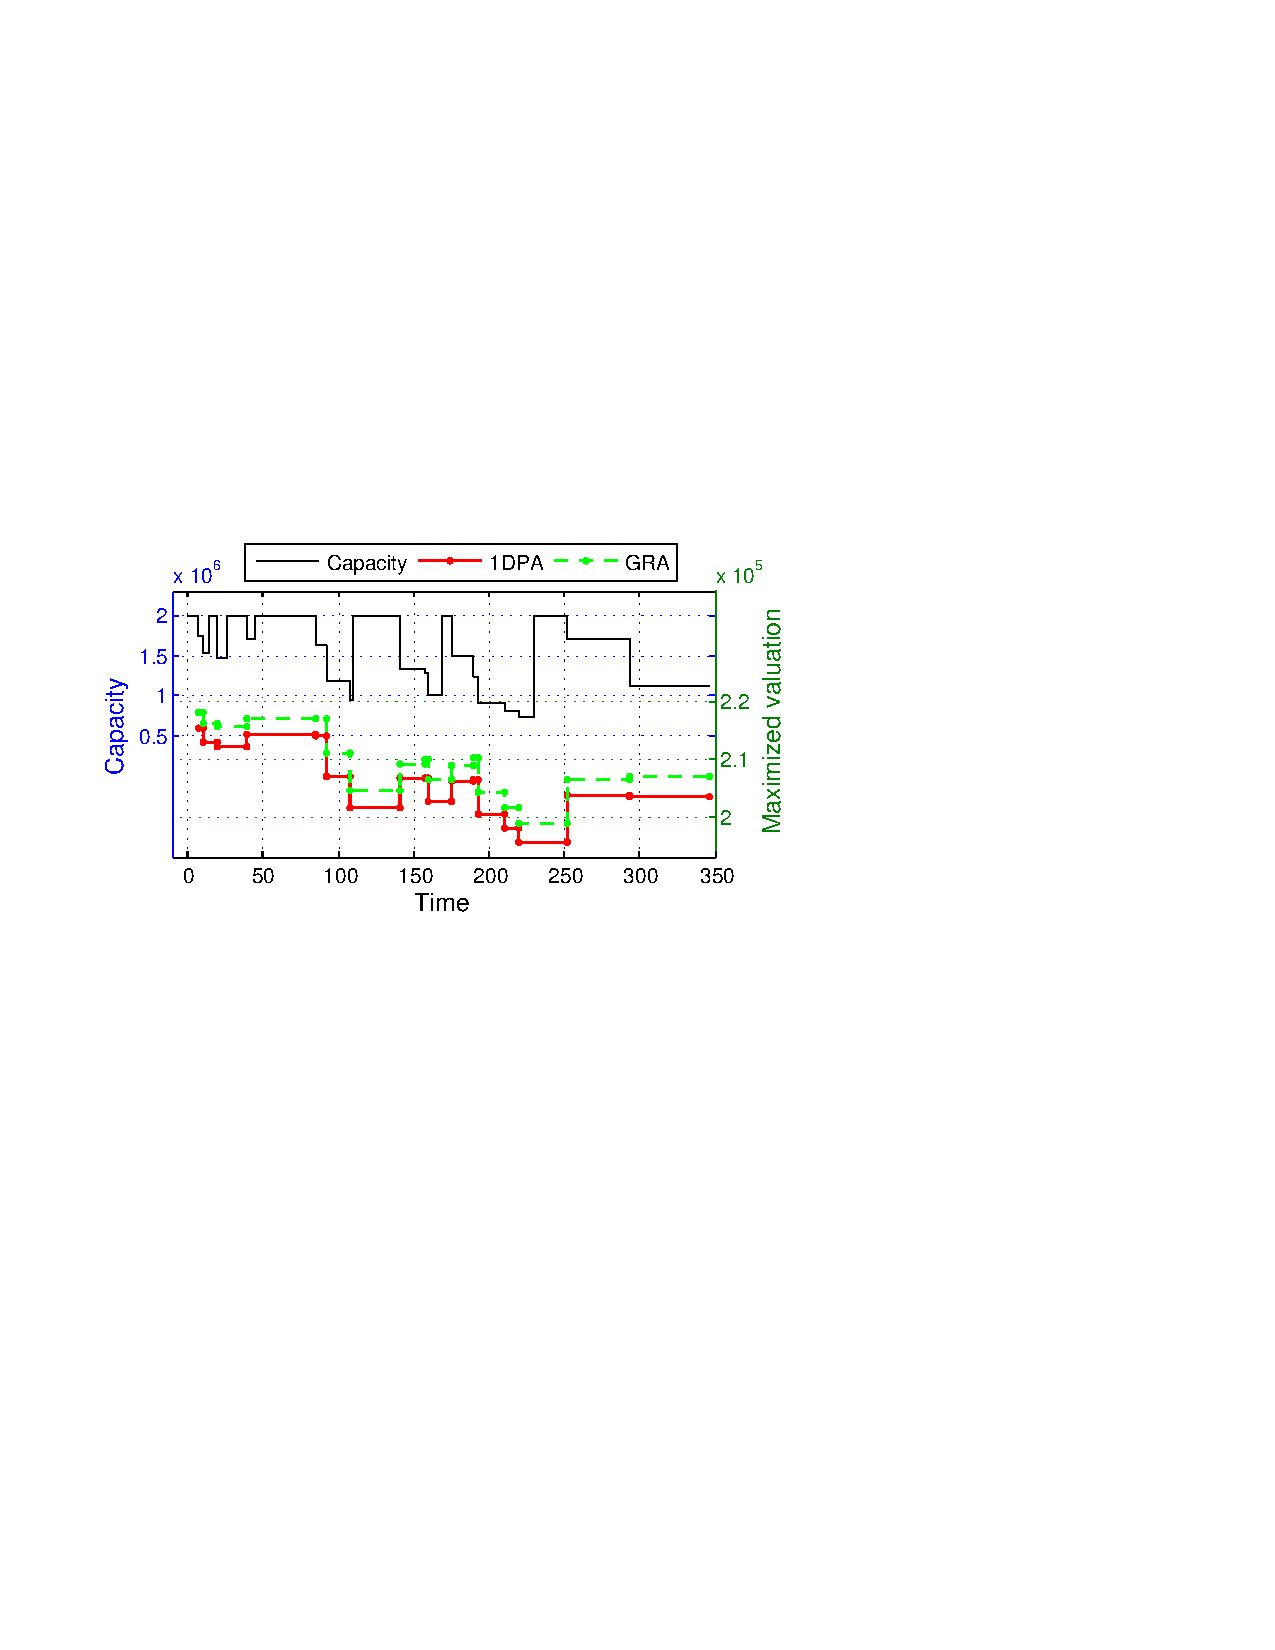
\includegraphics[scale=0.6]{fig/maxpatac.pdf}
	\end{center}\vspace{-5pt}
\caption{{\sc 1DPA} and {\sc GRA} apply to {\sc maxPA} with power-off protection constraint for Scenario FUR.}
	\label{fig:maxpatac}
\end{figure}

%\vspace{2mm}
One of the major parameters that evaluates an event-based demand response management algorithm is its running time. The algorithm should be sufficiently fast. Despite a considerable body of literature on this topic, however, they only considered microgrids with a significantly small number of customers, as compared to the number of customers considered in this paper. The running time with respect to a large number of customers is not studied.

Although in most cases {\sc 1DPA}'s solutions are remarkably close to the optimal, the running time is more than that of {\sc GRA}, especially in the scenarios with mixed customers. Generally, the more the number of customers, the larger is the running time, as seen from Fig.~\ref{fig:rt}.

Therefore, this paper proposes a two-stage hybrid approach to take advantage of both {\sc 1DPA} and {\sc GRA}.
\begin{figure}[!htb]
	\begin{center}
		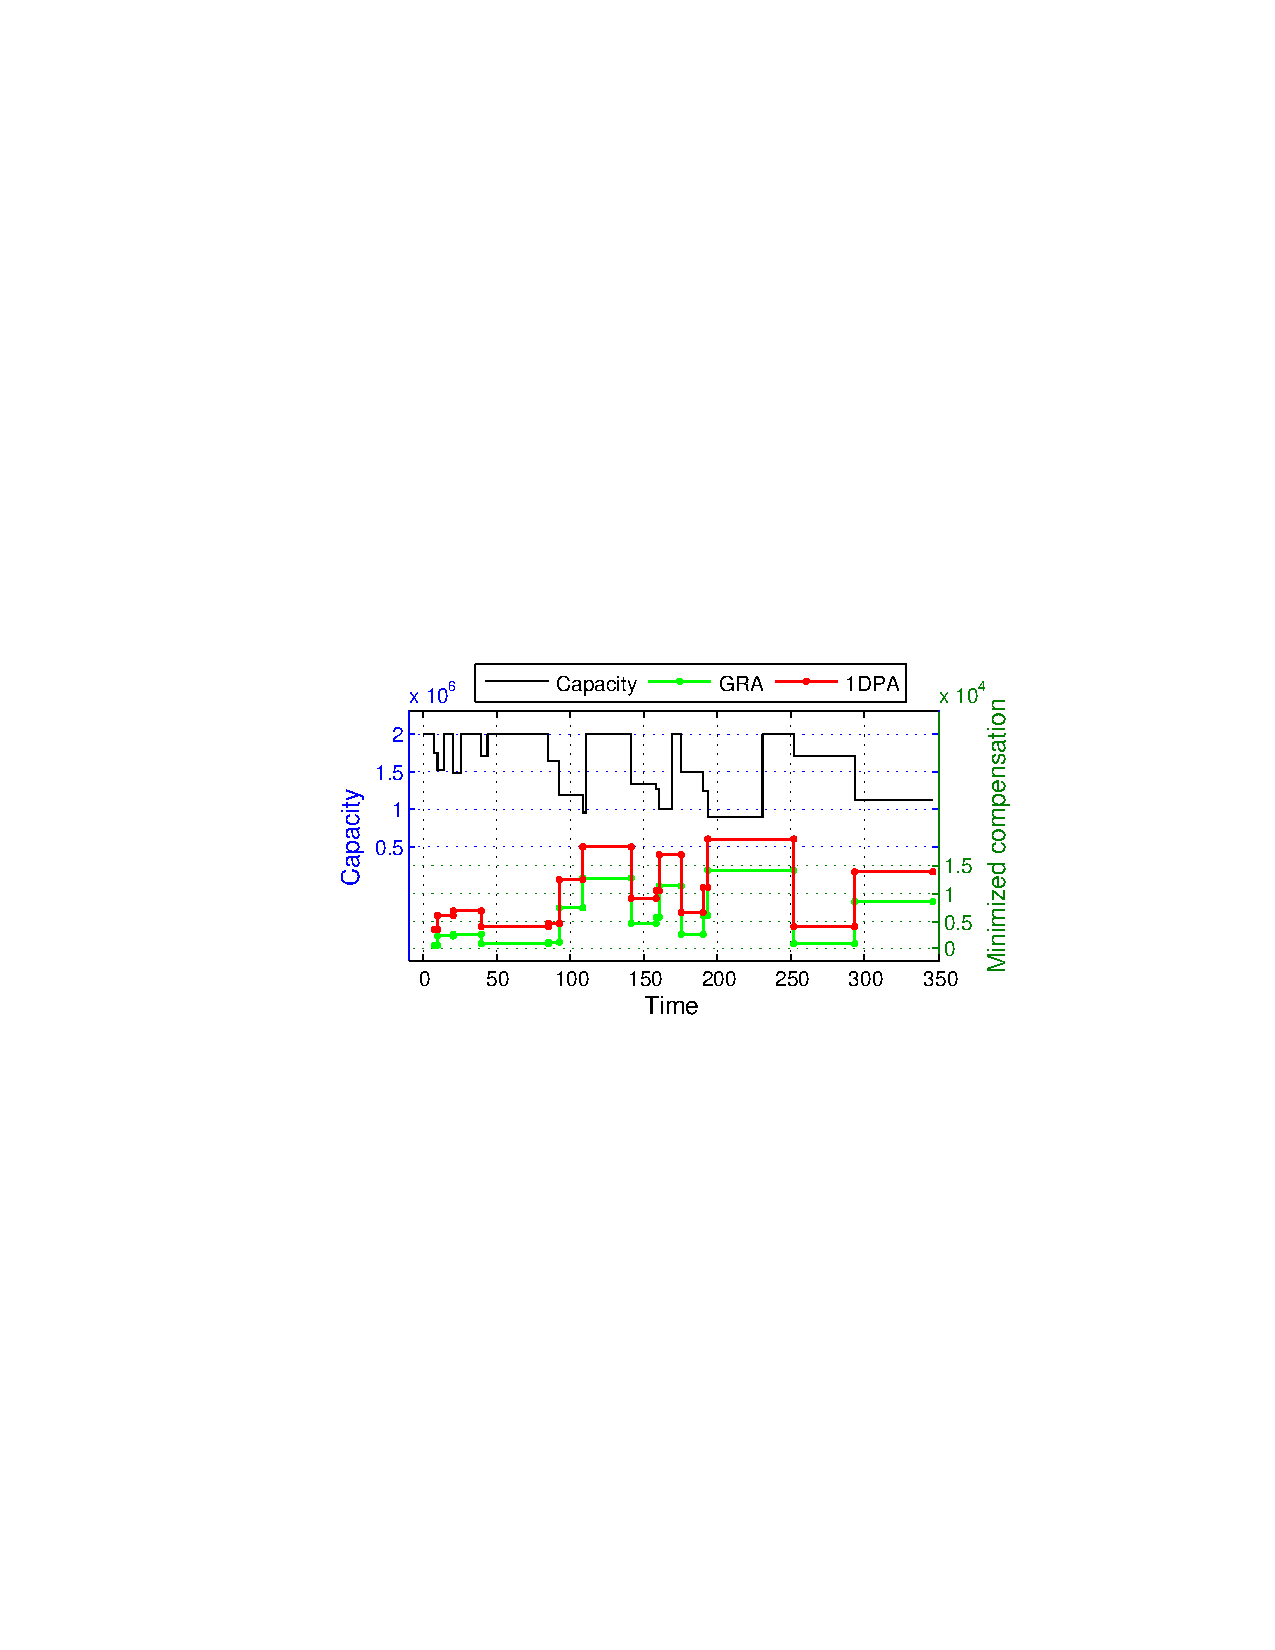
\includegraphics[scale=0.6]{fig/minpaac.pdf}
	\end{center}\vspace{-5pt}
\caption{{\sc 1DPA} and {\sc GRA} apply to {\sc minPA} without power-off protection constraint for Scenario FUR.}
	\label{fig:minpaac}
\end{figure}

\begin{figure}[!htb]\vspace{-5pt}
	\begin{center}
		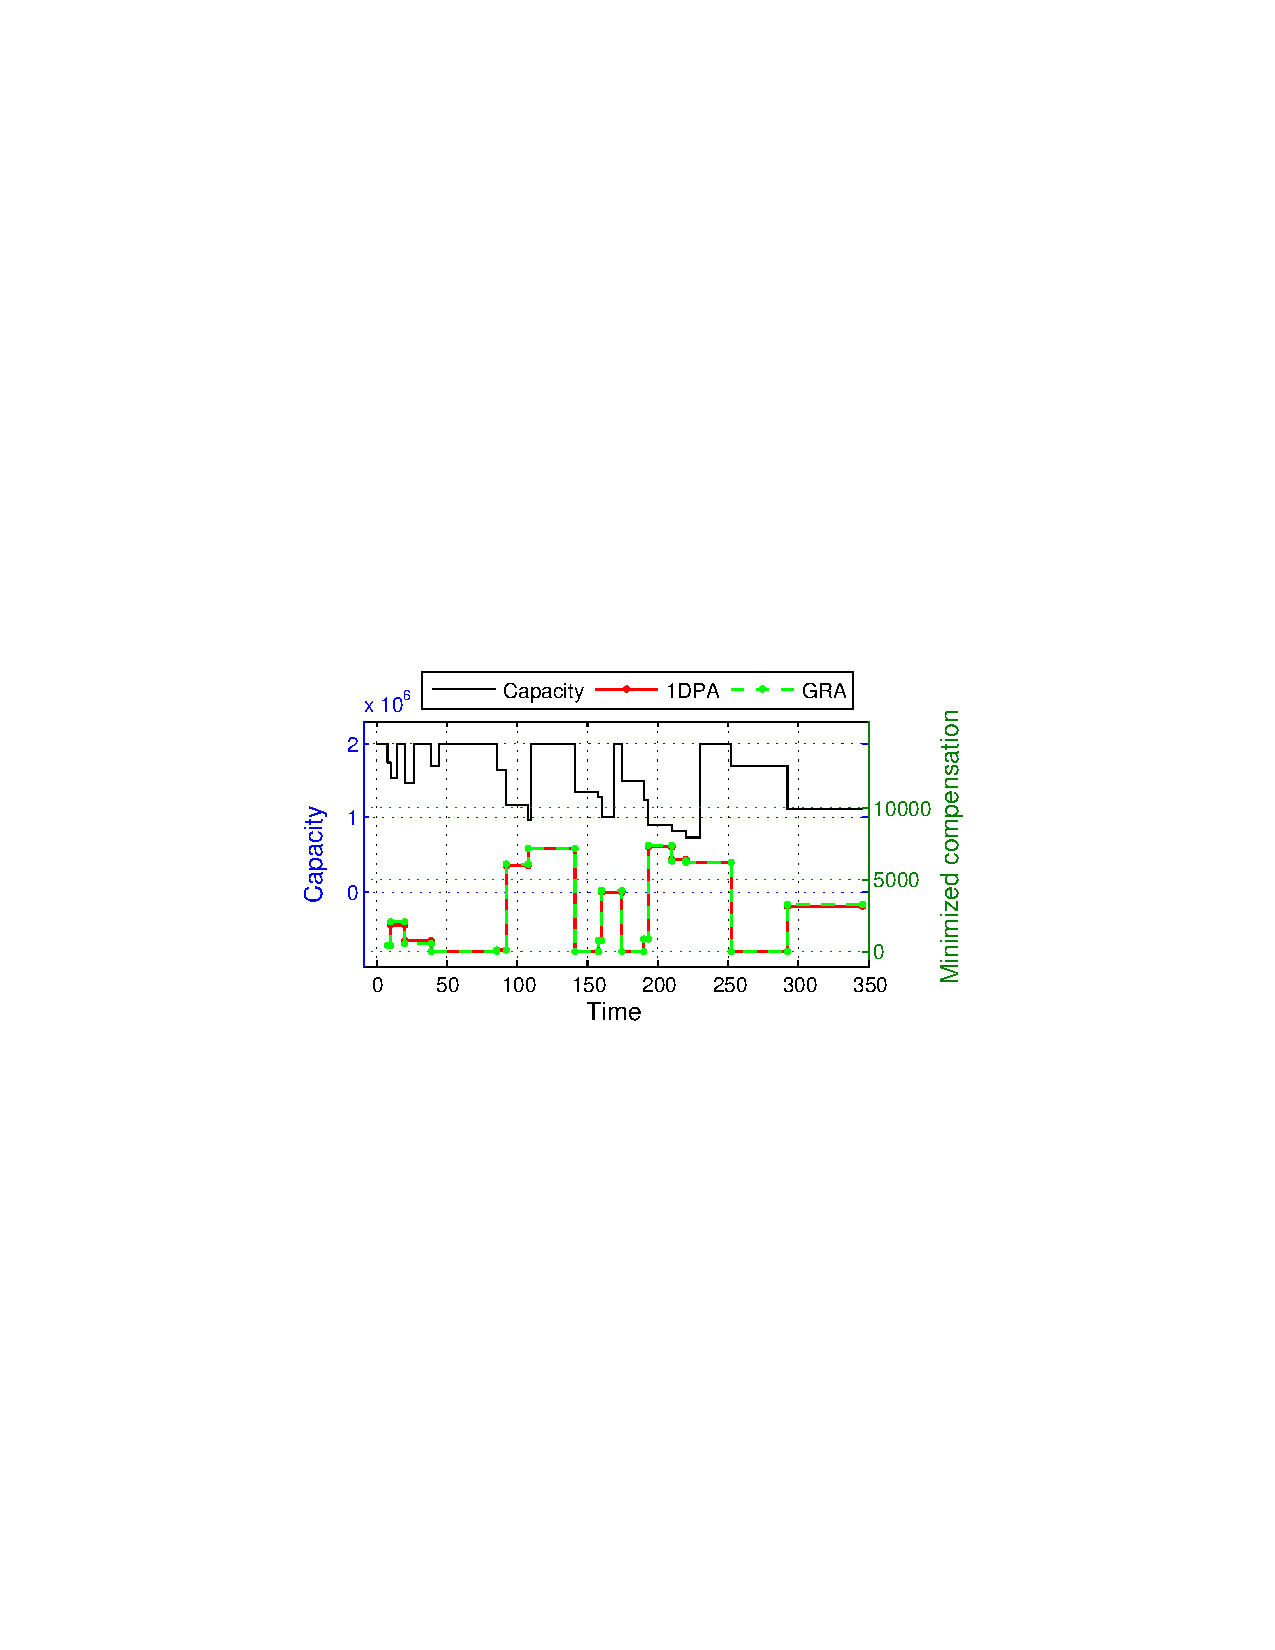
\includegraphics[scale=0.6]{fig/minpatdc.pdf}
	\end{center}\vspace{-5pt}
\caption{{\sc 1DPA} and {\sc GRA} apply to {\sc minPA} with power-off protection constraint for Scenario AUR.}
	\label{fig:minpatdc}
\end{figure}

 \vspace{-5pt}
\subsubsection{Dynamic Capacity}~\\


In addition to the aforementioned scenarios, simulations are performed considering the case when the microgrid's capacity is varying over time due to possible events (e.g., failure, or resumption), whereas the set of customers is fixed. 

The aforementioned scenario is applied to both {\sc maxPA} and {\sc minPA}  with and without power-off protection constraint. The events, namely Failure and Resumption, occur according to an exponential distribution with a n expected rate $200$. When the microgrid is in the Failure state, the capacity decreases randomly from $5\%-35\%$, whereas when in the Resumption state the microgrid's capacity is fully resumed (i.e.,  $C=$2MVA), except the times when an events occurred the remaining time the microgrid is in the Steady state (i.e., it remains at the same state as was in the previous). Whether an event is the Failure or Resumption state is determined according to a Markov chain with the following settings:
 \begin{enumerate}
 \item Steady $\rightarrow$ Failure with a probability of $65\%$
 \item Steady $\rightarrow$ Resumption with a probability of $35\%$
 \end{enumerate}
 
The value of $T^{\rm off}_k$ for each customer is generated randomly from a range $[0, |S_k| ]$. The results show that without power-off protection constraint for the scenarios with active power only, {\sc 1DPA} outperforms {\sc GRA} for both {\sc maxPA} and {\sc minPA}. In Fig.~\ref{fig:maxpa}, {\sc GRA}'s maximized valuation is lower than the one of {\sc 1DPA} and is constant. This is because {\sc GRA} simply fails to consider all the residential customers with small power demands as well as the remaining industrial customers whose power demand is relatively smaller compared to the industrial customers having considerably big power demand. For the other scenarios performance of {\sc 1DPA} and {\sc GRA} varies considerably based on the values of $T^{\rm off}_k$ as well as on customers' power demands' range, as seen from Figs.~\ref{fig:maxpatac},\ref{fig:minpaac},\ref{fig:minpatdc}.


 \vspace{-5pt}
\section{Conclusion}\label{sec:concl}

This paper presented efficient algorithms for event demand-based response in microgrid with provable approximation guarantee. 
A two-stage method was suggested that combines the advantages of two different approaches: the one-dimensional projection approach (1DPA) which guarantees a good approximation ratio but is computationally more demanding; and the greedy ratio approach (GRA) which is computationally very efficient, but has  worse approximation guarantee. This paper compares these methods with the methods currently used in practice, such as greedy utility, or greedy demand. The simulation results show the superiority of the suggested methods under various practical settings. The proposed approach can be applied to microgrid with a large number of customers.

%While GRA is worse than the 1DPA in terms of approximation guarantee, it has the advantage that it can be modified to work directly with the voltage and frequency fluctuations, i.e., without requiring an explicit value for the capacity. Investigating this further will be the subject of future work.  

\bibliographystyle{plain}
\bibliography{reference}

\vspace{-10pt}
\section{Appendix} \label{sec:append}

In the Appendix, the basic ideas of the proofs of Theorems~\ref{thm:alg-greedy}-\ref{thm:1dpa} are sketched.

\vspace{-10pt}
\subsection{Greedy Ratio Algorithm}

The basic idea of the proof of Theorem~\ref{thm:alg-greedy} is to compare the solution $X \cup \{j\}$ obtained by {\sc GRA} with the optimal solution. By the greedy order, each customer has a better or equal efficiency ratio than the corresponding optimum customer, when both the greedy and optimal solutions are considered according to the order $\frac{u_k}{|S_k|} \ge \frac{u_{k'}}{|S_{k'}|}$, when $k \le k'$. One can easily derive form this that the ratio of the total valuation of the set of customers in $X \cup \{j\}$ to the total valuation in any optimal set is bounded from below by the ratio of the sum of the absolutes of the demands in these two sets. It remains thus to bound  this ratio from below. This essentially amounts to relating the sum of the absolutes of a set vectors in $\CC$ to the absolute of the sum of these vectors, and can be shown by induction on the number of vectors. 

Fig.~\ref{fig:greedy} illustrates a tight extreme case when the optimum packs more power demands (in length) than that of {\sc GRA}. One can show by induction that the two  sides corresponding to $X^*$ (optimal sides) are equivalent (in the extreme case). Rescale all power demands such that each of the two optimal sides is equal to 1, then apply basic trigonometry 
$\sum_{k \in X \cup \{j\}}|S_k| = \sqrt{(1+\cos \theta)^2 + \sin^2 \theta} = \sqrt{2 + 2\cos \theta}$
Therefore, $\frac{\sum_{k \in X \cup \{j\} } |S_k|}{\sum_{k \in X^*} |S_k|} = \frac{\sqrt{2 + 2\cos \theta}}{2}=\sqrt{\frac{\cos \theta + 1}{2}}$
In this case, it follows that $u(X \cup \{j\}) \ge \sqrt{\frac{\cos \theta + 1}{2}} \cdot \OPT$. Finally, since the algorithm returns the maximum valuation of either $X$ or $\{j\}$, the solution objective is at least half of $X \cup \{j\}$.


\begin{figure}[!htb]
	\centering \vspace{-5pt}
		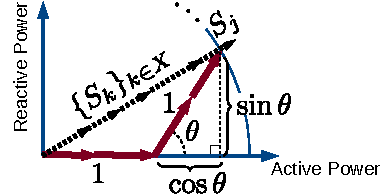
\includegraphics[scale=0.8]{fig/fig-greedy-brief.pdf} \vspace{-5pt}
\caption{The figure depicts an extreme case when the ratio  $\frac{\sum_{k \in X \cup \{j\}} | S_k|}{\sum_{k \in X^*} |S_k|}$ is minimal, where $X^*$ is an optimal solution. The dotted arrows represent solution $ X \cup \{j\}$ (which is infeasible), whereas the red solid arrows represent the optimal solution $X^*$. These two solutions constitute a triangle.}
	\label{fig:greedy}
\end{figure} 

\vspace{-20pt} 
\subsection{One-dimensional Projection Algorithm}

The basic idea of the proof of Theorem~\ref{thm:1dpa} is to divide the feasibility region into two parts: $\cD_1$ and $\cD_2$ (see Fig.~\ref{fig:proj}). There are three cases. (Case 1) If an optimal solution $X^*$ resides in $\cD_1$ (i.e., $\sum_{k \in X^*} S_k(t) \in \cD_1$), then it is equivalent to the classical knapsack problem with capacity $\frac{C}{\sqrt{2}}$, and ${\rm Alg}^{\rm kp}$ can find a close-to-optimal solution.  

(Case 2 and 3) On the other hand, if an optimal solution $X^*$ resides in $\cD_2$ (i.e., $\sum_{k \in X^*} S_k(t) \in \cD_2$), then one can show that it is either a singleton power demand with the maximum valuation, or a sum of power demands with at least half of valuation lies in $\D_1$ (which is equivalent to the classical knapsack problem with capacity $\frac{C}{\sqrt{2}}$). 

\begin{figure}[!htb]
\centering \vspace{-10pt}
\includegraphics[scale=0.60]{fig/{fig-0.5-proof2}.pdf} \vspace{-15pt}
\caption{The feasibility region is divided into $\cD_1$ and $\cD_2$. } 
\label{fig:proj}
\end{figure}

\end{document}
